\documentclass[12pt,a4paper,twoside]{ipb}

% Pacote para projeto (não usar em dissertação de mestrado)
\usepackage{projei}

% Idioma e codificação
\usepackage[portuguese]{babel}
\usepackage[utf8]{inputenc}

% Gestão de bibliografia com BibLaTeX
\usepackage[style=ieee,backend=biber]{biblatex}
\addbibresource{lib/refs.bib}

% Pacotes gráficos e visuais
\usepackage{graphicx}
\graphicspath{{./images/}}
\usepackage{color}
\usepackage[table,xcdraw]{xcolor}  % Corrigido sem conflitos

% Formatação e estrutura
\usepackage{geometry}
\geometry{a4paper, margin=2cm}
\usepackage{titlesec}
\usepackage{float}
\usepackage{tabularx}
\usepackage{tabulary}
\usepackage{array}
\usepackage{enumitem}
\usepackage{placeins}
\usepackage{needspace}
\usepackage{lipsum}
\usepackage{etoolbox}
\usepackage{pdfpages}

% Links
\usepackage{hyperref}
\hypersetup{
  colorlinks=true,
  urlcolor=black,
  linkcolor=black,
  citecolor=black,
  bookmarks=true,
  pdfstartview=FitH
}

% Listagens de código
\usepackage{listings}
\definecolor{codegray}{gray}{0.95}
\definecolor{yamlkey}{rgb}{0.0,0.0,0.6}
\definecolor{yamlstring}{rgb}{0.7,0.0,0.0}

\lstdefinelanguage{YAML}{
  keywords={true,false,null,y,n},
  keywordstyle=\color{yamlkey},
  basicstyle=\scriptsize\ttfamily,
  commentstyle=\color{gray},
  stringstyle=\color{yamlstring},
  morecomment=[l]{\#},
  morestring=[b]",
  morestring=[b]'
}

\lstset{
  inputencoding=ascii,
  basicstyle=\ttfamily\scriptsize,
  breaklines=true,
  breakatwhitespace=false,
  numbers=left,
  numberstyle=\tiny,
  captionpos=b,
  frame=single,
  xleftmargin=3.5em,
  framexleftmargin=3.5em,
  showstringspaces=false,
  columns=fullflexible,
  literate=
    {°}{{\textdegree}}1
    {á}{{\'a}}1
    {ã}{{\~a}}1
    {ç}{{\c{c}}}1
    {é}{{\'e}}1
    {º}{{\textordmasculine}}1
    {ê}{{\^e}}1
    {_}{{\_}}1
}

% Metadados do projeto
\title{Aplicação para controlo de casa inteligente, utilizando Home Assistant}
\author{José Guedes - a56576}
\secondauthor{Nelson Fernandes - a51796}
\supervisor{Prof. Pedro Filipe Fernandes Oliveira}
\cosupervisor{Prof. Paulo Matos}
\courseyear{2024-2025}

% Glossário
\makeglossaries
\loadglsentries{acronym}

\begin{document}

% Capas e prefácio
\beforepreface

\prefacesection*{Resumo}
%\thispagestyle{empty}

Vivemos numa época em que a sociedade está mais dependente da tecnologia, utilizando-a, por exemplo, para automatizar, controlar e gererir ambientes residenciais. A automação residencial, uma das áreas em maior crescimento a nível mundial, tem conquistado espaço ao oferecer soluções inovadoras que promovem conforto, segurança e eficiência nas habitações.

Este projeto visa o desenvolvimento de um sistema de automação residencial para integrar e centralizar diversos dispositivos e sistemas inteligentes, com o objetivo de melhorar o conforto, a segurança e a eficiência da habitação. A comunicação entre os dispositivos inteligentes é realizada exclusivamente através de conectividade Wi-Fi, garantindo uma configuração simples e sem fios.

Para isso, foi utilizada a plataforma \gls{HA}, que foi escolhida pela sua flexibilidade e capacidade de integrar uma ampla gama de dispositivos inteligentes, permitindo o controlo centralizado de diferentes sistemas. Além disso, foi utilizado o \gls{YAML} para a configuração e personalização do sistema, proporcionando uma maneira simples e legível de definir as integrações e automações. A combinação destas ferramentas permitiu o desenvolvimento de uma solução eficaz para o controlo inteligente de ambientes residenciais.


\mbox{}\linebreak
\noindent {\bf Palavras-chave:} home assistant, yaml, automação, ambientes inteligentes.


%\vfill
%\pagebreak
%\mbox{}
%\vfill
%\pagebreak

\prefacesection*{Abstract}
%\thispagestyle{empty}

We live in an era where society is increasingly dependent on technology, using it, for example, to automate, control, and manage residential environments. Residential automation, one of the fastest-growing sectors worldwide, is gaining traction by offering innovative solutions that promote comfort, security, and efficiency in homes.

This project aims to develop a residential automation system to integrate and centralize various smart devices and systems, with the goal of enhancing comfort, security, and efficiency in the home.

For this purpose, the \gls{HA} platform was used, chosen for its flexibility and ability to integrate a wide range of smart devices, enabling centralized control of different systems. Additionally, \gls{YAML} was utilized for system configuration and personalization, providing a simple and readable way to define integrations and automations. The combination of these tools enabled the development of an effective solution for intelligent control of residential environments.


\mbox{}\linebreak
\noindent {\bf Keywords:} home assistant, yaml, automation, smart environments.

%\vfill
%\pagebreak
%\mbox{}
%\vfill
%%\pagebreak

% Siglas
\afterpreface
\printglossary[type=\acronymtype,title={Siglas}]

% Corpo principal
\bodystart
\cleardoublepage \chapter{Introdução}\label{cap:intro}


A automação residencial tem-se destacado como uma área de grande potencial de crescimento, proporcionando aos moradores um maior controlo sobre as suas casas através de dispositivos conectados, oferecendo benefícios em termos de conveniência e gestão eficiente de recursos. Este projeto surge como uma contribuição para a evolução dessa área, ao desenvolver um sistema integrado de automação residencial que centraliza o controlo de diversos dispositivos inteligentes numa única plataforma.

\section{Enquadramento}

É inegável que, nos últimos anos, o mercado dos dispositivos inteligentes tem crescido a um ritmo acelerado. O aumento das soluções de domótica, impulsionado pela popularização das casas inteligentes e do interesse em controlar as habitações são das principais razões. Estes dispositivos inteligentes, cada vez mais, fazem parte do nosso quotidiano, melhorando a maneira como interagimos com a casa, proporcionando um maior conforto aos utilizadores, assim como uma gestão dos gastos energéticos e na segurança da habitação.
A instabilidade nos preços da energia e uma maior preocupação ambiental têm levado os consumidores a procurar soluções \gls{IoT} que permitam uma utilização mais racional dos recursos.

Apesar deste crescimento dos dispositivos \gls{IoT} e do elevado interesse das pessoas, muitos utilizadores ainda enfrentam dificuldades na integração e configuração com a plataforma escolhida. Muitas vezes existe falta de compatibilidade entre a plataforma escolhida e os dispositivos \gls{IoT}.

Para resolver estes problemas, surgiu o \gls{HA}, uma solução open-source que conta com uma vasta lista de dispositivos compatíveis e uma grande comunidade que desenvolve e mantém as integrações. Um dos pontos fortes desta plataforma é o facto de não depender de serviços externos, o que garante total privacidade e controlo dos dados.

Como já referido, uma das grandes vantagens do \gls{HA} é a sua comunidade ativa, sempre atualizando e disponibilizando novas e melhoradas soluções. Esta comunidade é fundamental para manutenção e evolução do \gls{HA}. Com o empenho desta comunidade, o \gls{HA} tornou-se uma das melhores opções para soluções de domótica, sendo extremamente estável, versátil e compatível com a maioria dos dispositivos existentes no mercado. Tudo isto tem atraído cada vez mais utilizadores e desenvolvedores à plataforma.


\section{Objetivos}

O foco deste projeto é demonstrar de uma maneira simples, a capacidade do \gls{HA} para criar um sistema de domótica simples e centralizado. Para isso criou-se um sistema que permite uma observação gráfica do consumo/produção de energia da casa, visualização das câmaras de segurança e um controlo das temperaturas através de termostatos. Desta forma, podemos garantir um maior conhecimento dos gastos de energia e um controlo da habitação.


\section{Estrutura do Documento}

O relatório está organizado da seguinte forma:
\begin{itemize}
  \item \textbf{Capítulo 1: Introdução} \\
  Apresenta o contexto do projeto, os seus objetivos e a estrutura geral do documento.

  \item \textbf{Capítulo 2: Contexto e Tecnologias/Ferramentas} \\
  Descreve as tecnologias utilizadas no desenvolvimento do sistema, com destaque para a plataforma \gls{HA} e a linguagem \gls{YAML}, explicando o seu papel na integração e personalização das automações.

  \item \textbf{Capítulo 3: Análise de Requisitos} \\
  Detalha o processo de implementação, desde a integração dos dispositivos inteligentes até à configuração das automações e personalização da interface gráfica.

  \item \textbf{Capítulo 4: Desenvolvimento/Implementação} \\
  Apresenta os resultados obtidos, acompanhados de uma análise crítica sobre o desempenho, usabilidade e eficácia da solução desenvolvida.

  \item \textbf{Capítulo 5: Conclusões} \\
  Resume as principais conclusões do projeto e sugere possíveis melhorias ou desenvolvimentos futuros com base na experiência adquirida.
\end{itemize}
\cleardoublepage \chapter{Contexto e Tecnologias/Ferramentas}\label{cap:conceptual}

\section{Estado da Arte}

A revisão da literatura destaca as principais soluções e tecnologias atualmente disponíveis na área de automação residencial:

\subsection*{Plataformas de Automação Residencial}
\begin{itemize}
    \item \textit{Home Assistant}: Plataforma \textit{open source} amplamente utilizada para automação residencial, conhecida pela sua flexibilidade e suporte a uma vasta gama de dispositivos e serviços.
    \item \textit{SmartThings}: Plataforma da Samsung que permite integração com dispositivos inteligentes, mas com maior dependência de serviços baseados em nuvem.
    \item \textit{OpenHAB}: Outra solução \textit{open-source} focada em integrar dispositivos diversos, mas com uma curva de aprendizado mais acentuada.
\end{itemize}

\subsection*{Tecnologias Subjacentes}
\begin{itemize}
    \item \textbf{Protocolos de Comunicação}: Tecnologias como \textit{Zigbee}, \textit{Z-Wave} e \textit{MQTT} são amplamente utilizadas para conectar dispositivos de forma confiável e eficiente.
    \item \textbf{Assistentes Virtuais}: A integração com assistentes como a Alexa permite o controlo por comandos de voz, aumentando a usabilidade e acessibilidade do sistema.
\end{itemize}


\section{Tecnologias e Ferramentas Utilizadas}

\subsection*{Linguagem YAML}

A linguagem \gls{YAML} será utilizada para configurar e definir as automações e integrações do \gls{HA}. 
As principais características que justificam sua escolha incluem:

\begin{itemize}
    \item \textbf{Simplicidade e Legibilidade:} a sintaxe intuitiva e minimalista facilita a criação de configurações complexas.
    \item \textbf{Estrutura Hierárquica:} ideal para definir dependências e relações entre dispositivos e automações.
    \item \textbf{Compatibilidade com o Home Assistant:} \gls{YAML} é a linguagem padrão para configurar o \gls{HA}, sendo amplamente documentada e suportada.
\end{itemize}

\subsection*{Comunicação via Wi-Fi}

Os dispositivos inteligentes utilizados no sistema (como medidores de consumo \textit{Shelly}, câmaras, termostatos, estores, entre outros) comunicam-se entre si e com o \gls{HA} através da rede Wi-Fi da casa. Esta tecnologia desempenha um papel fundamental por:

\begin{itemize}
    \item  Eliminar a necessidade de cabos adicionais;
    \item Permitir controlo e monitorização remotos dos dispositivos;
    \item Facilitar a integração com a infraestrutura de rede já existente.
\end{itemize}

O uso do Wi-Fi como meio de comunicação garante uma instalação flexível, reduz os custos com infraestrutura e torna possível o acesso aos dados e controlo da casa inteligente a partir de qualquer lugar com ligação à Internet.

\section{Vantagens/Desvantagens do Home Assistant}

As principais vantagens do \gls{HA} incluem:

\begin{itemize}
    \item \textbf{Código Aberto:} Permite personalizações avançadas e liberdade para adaptações específicas.
    \item \textbf{Compatibilidade Ampla:} Suporte para milhares de dispositivos e protocolos, como \textit{Zigbee, Z-Wave e MQTT}.
    \item \textbf{Autonomia Local:} Funciona de forma independente da nuvem, priorizando privacidade e segurança.
    \item \textbf{Flexibilidade:} Possibilita automações complexas e personalizadas, adaptadas às necessidades.
    \item \textbf{Custo-Benefício:} Gratuito e com uma vasta comunidade de suporte, reduzindo custos de manutenção.
    \item \textbf{Atualizações Constantes:} A comunidade ativa proporciona melhorias regulares e novos recursos.
\end{itemize}

As principais desvantagens do \gls{HA} incluem:

\begin{itemize}
    \item \textbf{Grau de dificuldade inicial:} Pode ser desafiador para iniciantes devido à necessidade de configurar arquivos \gls{YAML} e aprender conceitos técnicos.
    \item \textbf{Dependência de Hardware Local:} Requer um dispositivo dedicado (como \textit{Raspberry Pi} ou similar) para operação, o que pode aumentar os custos iniciais.
    \item \textbf{Complexidade de Configuração:} Algumas integrações e automações avançadas podem ser difíceis de implementar sem conhecimento técnico prévio.
    \item \textbf{Manutenção Regular:} Atualizações frequentes podem introduzir mudanças que exigem ajustes na configuração existente.
    \item \textbf{Desempenho em Sistemas Grandes:} Em implementações extensas, o desempenho pode ser afetado sem hardware adequado.
\end{itemize}


\section{Plataformas Relacionadas}

\subsection{OpenHAB}

O \textit{OpenHAB} é uma plataforma \textit{open-source} dedicada à automação residencial, semelhante ao \gls{HA}. Foi uma das primeiras soluções deste género a surgir no mercado, com uma arquitetura modular que suporta diversos protocolos de comunicação, como o \textit{Z-Wave}, \textit{Zigbee} e \textit{MQTT}. No entanto, apresenta uma curva de aprendizagem mais acentuada, sendo necessário um conhecimento técnico mais aprofundado para realizar configurações e integrações.

Em comparação com o projeto desenvolvido, o \textit{OpenHAB} revela-se menos acessível para novos utilizadores e com uma interface menos moderna. Apesar disso, ambos partilham o objetivo de integrar e controlar dispositivos inteligentes de forma centralizada, mantendo o funcionamento local e sem depender de serviços na nuvem. O \gls{HA}, no entanto, destaca-se pela comunidade ativa e pela facilidade na personalização de dashboards, o que foi amplamente explorado neste trabalho.


\subsection{Domoticz}

O \textit{Domoticz} é uma plataforma leve para automação residencial, ideal para dispositivos com poucos recursos, como o \textit{Raspberry Pi}. Foca-se em fornecer funcionalidades básicas de controlo e monitorização de sensores, atuadores, luzes e outras entidades. A sua interface gráfica é simples, mas menos atrativa e intuitiva quando comparada ao \gls{HA}.

No contexto deste projeto, o Domoticz apresenta limitações em termos de integração com equipamentos modernos como câmaras \textit{Reolink}, bombas de calor \textit{Daikin}, sensores \textit{Netatmo} ou aspiradores \textit{iRobot}, o que o coloca em desvantagem em cenários mais complexos. Ainda assim, tal como o \gls{HA}, permite automação local e contribui para a independência de soluções baseadas em cloud. Para casos mais simples ou com restrições de hardware, pode ser uma opção viável.


\cleardoublepage \chapter{Análise de Requisitos}\label{cap:metodology}

Serve o presente capitulo para demonstrar todos os requisitos ao longo do desenvolvimento deste projeto.


\section{Modelação do Sistema de Automação Residencial}

Para iniciar o desenvolvimento do projeto, foi realizado um levantamento de todos os dispositivos, seguido do desenho de um diagrama de comunicação entre eles. A comunicação ocorre exclusivamente pela rede Wi-Fi local, garantindo conectividade direta e privada. A arquitetura do sistema e as conexões entre os dispositivos são mostradas na Figura~\ref{fig:Diagram_HA_2.png}, que integra produção e armazenamento de energia, carregamento de veículos elétricos, ar-condicionado, vigilância, controlo de estores, sensores ambientais \textit{Netatmo} e monitorização de energia, centralizados por meio da plataforma \gls{HA}. Para suportar essa infraestrutura, o \gls{HA} foi instalado numa máquina virtual no \textit{VirtualBox}, criando assim um ambiente controlado e isolado para testes e integração dos dispositivos. Esta abordagem proporcionou maior flexibilidade, facilidade de backup e segurança no processo de desenvolvimento do sistema de automação residencial.



\begin{figure}[H]
    \centering
    \includegraphics[width=\textwidth]{images/Diagram_HA_2.png}
    \caption{Diagrama do cenário de aplicação}
    \label{fig:Diagram_HA_2.png}
\end{figure}


\subsection{Visão Geral}

O diagrama representa um sistema integrado de \textbf{produção, monitorização e gestão de energia}, \textbf{ar condicionado}, \textbf{carregamento de veículos elétricos}, \textbf{videovigilância} e \textbf{automatização residencial}, centralizado no \gls{HA}.

\vspace{1em}
\subsection{Produção e Armazenamento de Energia}

À esquerda do diagrama encontram-se os módulos fotovoltaicos \textit{PV 1}, \textit{PV 2} e \textit{PV 3} (\textit{AXITEC}), responsáveis por captar a energia solar. Estes painéis estão ligados ao \textit{inversor - SUN2000-Master} (modelo \textit{Huawei}), que converte a corrente contínua (DC) gerada pelos painéis em corrente alternada (AC), utilizável na rede elétrica da casa.

O \textit{inversor - SUN2000-Master} está também ligado à bateria - \textit{Luna2000}, permitindo armazenar o excesso de energia solar para consumo posterior. Adicionalmente, este inversor está ligado à rede \textit{elétrica}, permitindo consumir energia da rede ou injetar excedente.

O sistema conta ainda com um inversor - \textit{SUN2000-Slave}, integrado na arquitetura para balanceamento e controlo eficiente. Toda esta infraestrutura é monitorizada via a integração \textit{Huawei}, possibilitando uma gestão centralizada dos fluxos energéticos.

\vspace{1em}
\textbf{Monitorização de Consumos}

Vários dispositivos \textit{Shelly EM} foram instalados para monitorizar consumos elétricos específicos. Um destes dispositivos mede o consumo geral da casa, outros monitorizam equipamentos individuais como:

\begin{itemize}
  \item Carregador de veículos elétricos \textit{Porsche};
  \item Bomba de calor \textit{(Daikin EABX-D6V)};
  \item Bomba de A.Q.S \textit{(Daikin EKHHP500AA2V3)};
  \item Carregador de veículos elétricos \textit{Huawei SCharger};
  \item \textit{Reolink} NVR e Câmaras;
\end{itemize}

A integração com a \textit{Shelly Integration} permite visualizar em tempo real os consumos e criar automações inteligentes, otimizando a utilização da energia produzida.

Além disso, um módulo \textit{Shelly 2.5} está ligado aos \textit{Blinds} (estores), permitindo a sua automação com base em condições como a produção solar, temperatura ou hora do dia. Através do \gls{HA}, os estores podem ser abertos ou fechados automaticamente para otimizar o conforto térmico e/ou a eficiência energética da casa.

\textbf{Aquecimento e Águas Quentes}

Os equipamentos de climatização \textit{Daikin} incluem a \textit{Heat Pump} para aquecimento e a \textit{A.Q.S Pump} para águas quentes sanitárias. Ambos estão integrados no sistema via \textit{DAIKIN Integration}, o que permite uma gestão eficiente, aproveitando preferencialmente a energia solar para funcionamento destes equipamentos.

\vspace{1em}
\textbf{Carregadores de Veículos Elétricos}

A arquitetura inclui dois carregadores:
\begin{itemize}
  \item Carregador \textit{Porsche} (carregador móvel);
  \item \textit{Huawei SCharger (modelo SCharger-7KS-S0);}
\end{itemize}

Estes carregadores estão ligados à rede da casa e monitorizados por dispositivos \textit{Shelly EM}, permitindo controlar e automatizar os carregamentos com base em horários de tarifa reduzida ou excedente solar.

\vspace{1em}
\textbf{Videovigilância}

O sistema de segurança é assegurado por \textit{câmaras} ligadas ao \textit{Reolink NVR}, que permite gravação e monitorização contínua. A integração via \textit{Reolink Integration} disponibiliza visualizações e alertas centralizados no \gls{HA}.

\vspace{1em}
\textbf{Meteorologia Inteligente e Controlo Ambiental}

O sistema inclui sensores da \textit{Netatmo}, integrados via \textit{Netatmo Integration}, nomeadamente:

\begin{itemize}
  \item \textit{Smart Weather Station – exterior};
  \item \textit{Smart Weather Station – interior;}
  \item \textit{Rain gauge;}
  \item \textit{Wind gauge;}
  \item \textit{Smart Indoor Camera;}
\end{itemize}

Estes dispositivos permitem recolher dados sobre temperatura, humidade, qualidade do ar, precipitação e presença no interior da casa. Esta informação é utilizada para ajustar automaticamente equipamentos como a climatização, estores ou alertar o utilizador de condições ambientais adversas.

\vspace{1em}
\textbf{Limpeza Autónoma}

O sistema integra ainda aspiradores inteligentes \textit{iRobot}, conectado via \textit{iRobot Integration}, que permite iniciar sessões de limpeza automáticas ou programadas com base em condições específicas, como ausência de pessoas na casa ou dias de maior produção solar.




\section{Equipamentos}

Nas subseções seguintes são descritas as funções e detalhes dos equipamentos.\

A \textit{Daikin EKHHP500AA2V3} é uma bomba de calor que produz água quente sanitária, onde a energia do ar exterior é utilizada para a aquecer. Isto torna-a mais eficiente e sustentável do que os sistemas tradicionais elétricos ou a gás. A \textit{Daikin EABX-D6V}, por outro lado, é uma unidade interior de bomba de calor que é utilizada para aquecimento, água quente sanitária (AQS) e sistemas de arrefecimento.

Esta unidade transfere energia térmica para o sistema de aquecimento ou AQS através da energia térmica da unidade exterior e permite a produção de água quente sanitária. Para vigilância, a \textit{Reolink NVR} é um gravador de vídeo em rede que suporta até 36 câmaras IP ao mesmo tempo, e também permite monitorizar e gerir as câmaras, tornando-o ideal para instalações de vigilância de grande dimensão.

No entanto, a \textit{Reolink RLC-811A} é uma câmara de segurança IP adequada para uso exterior, mas que também pode ser útil em interiores. É alimentada por PoE, tornando a instalação fiável e eficiente. No campo da energia solar, a \textit{Huawei SUN2000} é um inversor solar residencial com uma potência nominal de 5 kW, adequado para instalações residenciais ou de pequena escala. Oferece elevada eficiência e funciona com baterias, incluindo ainda monitorização inteligente. A \textit{Huawei LUNA2000} é uma bateria modular de iões de lítio que armazena o excesso de energia solar, permitindo o uso da energia armazenada durante a noite ou quando a produção é reduzida, aumentando assim o autoconsumo de energia e reduzindo a dependência da rede elétrica.

Os \textit{AXITEC AXIpremium XL HL} são painéis solares fotovoltaicos com células monocristalinas de alta eficiência e tecnologia half-cell. Estes painéis têm melhor desempenho em condições de sombra parcial, são mais duráveis e adequados para instalações que priorizam potência e eficiência. Para mobilidade elétrica, o \textit{Huawei SCharger} é um carregador de 7.2 kW para veículos elétricos que permite um carregamento rápido e seguro, integrando-se facilmente com sistemas fotovoltaicos para priorizar a energia solar no carregamento.

O \textit{Porsche Mobile Charger Connect} é um carregador inteligente e portátil para veículos elétricos que permite o carregamento em casa ou em diferentes locais através de tomadas domésticas ou industriais. Pode ser utilizado como uma solução móvel ou instalado permanentemente, incluindo ainda conectividade de rede para gestão remota e integração com sistemas de casa inteligente.

Para automação e controlo, foram utilizados dispositivos do ecossistema \textit{Shelly}. O \textit{Shelly 1PM Gen4} foi instalado para controlar o portão da garagem, permitindo a sua abertura e fecho de forma remota através da interface do \gls{HA}. Adicionalmente, foram instalados vários módulos \textit{Shelly 2.5} para o controlo dos estores elétricos, permitindo tanto o controlo manual como automatizado, totalmente integrado no painel de controlo.

Para o controlo climático interior, foram instalados cinco termóstatos inteligentes com fios \textit{TADO}. Estes dispositivos permitem a monitorização e regulação em tempo real da temperatura e humidade em várias divisões, oferecendo modos de aquecimento e arrefecimento configuráveis e integração total com o sistema central de automação.

Por fim, o sistema de monitorização ambiental baseia-se em quatro dispositivos da \textit{Netatmo}: a \textit{Netatmo Weather Station}, \textit{a Netatmo Smart Indoor Camera}, \textit{o Netatmo Wind Gauge e o Netatmo Rain Gauge}. Este conjunto permite a monitorização contínua da pressão atmosférica, níveis de ruído e concentração de dióxido de carbono, melhorando o conforto do utilizador e a gestão da qualidade do ar, com visualização dos dados no painel principal.



\section{Requisitos do Home Assistant e Hardware}

Para executar o \gls{HA}, os requisitos mínimos de hardware são os seguintes , dependendo do método de instalação:

\begin{itemize}
    \item \textbf{Máquina virtual (VM):}
    \begin{itemize}
        \item Pelo menos 2\,CPU cores;
        \item 2\,GB RAM (4\,GB são recomendados para uma melhor performance);
        \item 32\,GB de espaço do disco;
        \item Adaptador de rede com acesso à internet.
    \end{itemize}
    
    \item \textbf{Raspberry Pi:}
    \begin{itemize}
        \item Raspberry Pi 4 (2\,GB mínimo, 4\,GB ou 8\,GB recomendado);
        \item cartão microSD (32\,GB minimo, ou SSD via USB para maior fiabilidade.);
        \item Power supply (3A USB-C official recomendado);
        \item Ligação Ethernet ou Wi-Fi.
    \end{itemize}
\end{itemize}


\section{Dashboards a Desenvolver}

Com o objetivo de garantir o cumprimento de todos os requisitos funcionais definidos, foi desenvolvido um conjunto de dashboards temáticos, cada um focado numa funcionalidade específica do sistema de automação residencial. Estes dashboards permitem uma visualização clara e intuitiva do estado dos dispositivos, bem como o controlo direto sobre os mesmos.

Entre os dashboards a implementar, destacam-se os seguintes:
\begin{itemize}
    \item \textbf{Dashboard Principal}: servirá como ecrã de entrada e terá como função apresentar, de forma resumida e centralizada, as informações mais relevantes dos vários sistemas integrados, como temperatura ambiente, consumo energético atual, estado das câmaras, entre outros.
    \item \textbf{Dashboard Energia}: permitirá a monitorização detalhada da produção e consumo energético, integrando dados provenientes do inversor solar, baterias, carregadores de veículos elétricos, e dispositivos \textit{Shelly}.
    \item \textbf{Dashboard Bombas}: focada na gestão das bombas de calor e do sistema de AQS (Águas Quentes Sanitárias), com possibilidade de ajuste de temperaturas e modos de operação em tempo real.
    \item \textbf{Dashboard Câmaras}: dedicada ao acompanhamento em tempo real das câmaras de segurança, permitindo uma visão geral de todas as zonas exteriores da casa.
    \item \textbf{Dashboard Estores}: facilitará o controlo manual e automático de todos os estores elétricos da habitação, com indicação da posição atual de cada um.
    \item \textbf{Dashboard Netatmo}: mostrará dados de sensores ambientais (temperatura, humidade, pressão atmosférica, ruído, CO\textsubscript{2}), recolhidos pelos dispositivos \textit{Netatmo}, promovendo o conforto e qualidade do ar interior.
    \item \textbf{Dashboard iRobot}: mostrará todos os dispositivos \textit{iRobot} que foram integrados.
\end{itemize}

Cada dashboard será desenhada com foco na usabilidade, garantindo uma interface limpa, responsiva e adaptada às necessidades do utilizador, promovendo um controlo total da casa inteligente a partir de um único sistema integrado.

\newpage

\section{Requisitos Funcionais}

\begin{table}[h!]
\centering
\resizebox{!}{11.5cm}{
\rowcolors{2}{gray!10}{white}
\begin{tabularx}{\textwidth}{|X|p{2.5cm}|>{\raggedright\arraybackslash}X|p{2.1cm}|p{2.1cm}|}
\hline
\textbf{Funcionalidade} & \textbf{Sensor} & \textbf{Entidade} & \textbf{Integração} & \textbf{Dashboard} \\
\hline
Verificar temperatura da sala & Tado sala & sensor. sala\_temperatura & Tado & Main e TADO \\

Verificar humidade da sala & Tado sala & sensor. sala\_humidade & Tado & Main e TADO \\

Verificar temperatura da suite & Tado suite & sensor. suite\_temperatura & Tado & Main e TADO \\

Verificar humidade da suite & Tado suite & sensor. suite\_humidade  & Tado & Main e TADO \\

Verificar temperatura do quarto RC & Tado quarto RC & sensor. quartorc\_temperatura & Tado & Main e TADO \\

Verificar humidade do quarto RC & Tado quarto RC & sensor. quartorc\_humidade & Tado & Main e TADO \\

Verificar temperatura do quarto Nascente & Tado quarto Nascente & sensor. quartonascente\_temperatura & Tado & Main e TADO \\

Verificar humidade do quarto Nascente & Tado quarto Nascente & sensor. quartonascente\_humidade & Tado & Main e TADO \\

Verificar temperatura do quarto Poente & Tado quarto Poente & sensor. quartopoente\_temperatura & Tado & Main e TADO \\

Verificar humidade do quarto Poente & Tado quarto Poente & sensor. quartopoente\_humidade & Tado & Main e TADO \\

Verificar temperatura exterior & Netatmo-Exterior & sensor. netatmo\_1piso\_ netatmo\_ exterior\_temperature & Netatmo & Main e  Netatmo \\

Verificar humidade exterior & Netatmo-Exterior & sensor. netatmo\_1piso\_ netatmo\_ exterior\_humidity & Netatmo & Main e   Netatmo \\

Verificar precipitação atual & Netatmo-Exterior & sensor. netatmo \_1piso\_rain\_ gauge\_precipitation & Netatmo & Main e Netatmo \\

Verificar precipitação total diária & Netatmo-Exterior & sensor. netatmo \_1piso\_rain\_ gauge\_precipita-tion\_today & Netatmo & Main e Netatmo \\

Verificar velocidade do vento & Netatmo-Anemómetro Inteligenter & sensor. netatmo \_1piso\_anenometer\_ wind\_speed & Netatmo & Main e Netatmo \\

Verificar direção do vento & Netatmo-Anemómetro Inteligente & sensor. netatmo \_1piso\_anenometer\_ wind\_direction & Netatmo & Main e Netatmo \\

Abrir/Fechar portao da Garagem & Shelly-Garage\_ Door & climate. altherma\_leaving\_ water\_tempera-ture & Shelly & Main \\

Verificar o estado e power da bateria & Huawei-State of capacity & sensor.batteries\_ state\_of\_ capacity & Huawei & Main e Energy \\

Verificar produção solar & Huawei (...) & sensor.solar\_total & Huawei & Main e Energy \\

Verificar power da rede & Shelly-Medidor Geral & sensor.rede\_power & Shelly & Main e Energy \\


\hline
\end{tabularx}
}
\caption{Funções, sensores e entidades no sistema}
\end{table}


\begin{table}[h!]
\centering
\resizebox{!}{11cm}{
\rowcolors{2}{gray!10}{white}
\begin{tabularx}{\textwidth}{|X|p{2.5cm}|>{\raggedright\arraybackslash}X|p{2.1cm}|p{2.1cm}|}
\hline
\textbf{Funcionalidade} & \textbf{Sensor} & \textbf{Entidade} & \textbf{Integração} & \textbf{Dashboard} \\
\hline
Verificar consumo da bomba AQS & Shelly-Bomba\_AQS & sensor.bomba\_aqs\_fil-tered\_power & Shelly & Main e Energy \\

Verificar consumo da bomba de calor & Shelly-Bomba\_Calor & sensor.bomba\_calor\_ filtered\_power & Shelly & Main e Energy \\

Verificar consumo do EV16 & Shelly-EV\_16A & sensor.ev\_16\_ filtered\_power & Shelly & Main e Energy \\

Verificar consumo do EV32 & Shelly-EV\_32A & sensor.ev\_32\_ filtered\_power & Shelly & Main e Energy \\

Verificar estado do robo Roomba\_Sala & iRobot-Roomba\_Sala & vacuum.roomba\_sala & iRobot & Main e iRobot \\

Verificar estado do robo Braava\_Sala & iRobot-Braava\_Sala & vacuum.braava\_sala & iRobot & Main e iRobot \\

Verificar estado do robo Roomba\_Piso & iRobot-Roomba\_Piso & vacuum.roomba\_piso & iRobot & Main e iRobot \\

Verificar estado do robo Roomba\_Bunker & iRobot-Roomba\_Bunker & vacuum.roomba\_bunker & iRobot & Main e iRobot \\

Verificar estado do robo Roomba\_Cave & iRobot-Roomba\_Cave & vacuum.roomba\_cave & iRobot & Main e iRobot \\

Baixar/Subir estore do quarto Nascente & Shelly-Quarto\_Nas-cente & cover.quarto\_nascente & Shelly & Blinds \\

Monitorizar a camara 1 & Reolink-Camara1 & camera.camara1\_trans-parente & Reolink & NVR \\

Monitorizar a camara da frente & Reolink-Frente-1 & camera. frente\_1\_trans-parente & Reolink & Main e NVR \\

Monitorizar a camara da garagem & Reolink-Garagem-1 & camera. garagem\_8\_transparente & Reolink & Main e NVR \\

Monitorizar a camara das escadas & Reolink-Escadas-4 & camera.escadas\_4\_ transparente & Reolink & NVR \\

Monitorizar a camara da piscina & Reolink-Piscina-5 & camera.piscina\_5\_ transparente & Reolink & NVR \\

Monitorizar a camara da platibanda & Reolink-Platibanda-5 & camera.platibanda\_6\_ transparente & Reolink & NVR \\

Monitorizar a camara da rampa norte & Reolink-Rampa-Norte-3 & camera.rampa\_norte\_ 3\_transparente & Reolink & NVR \\

Monitorizar a camara da rampa sul & Reolink-Rampa-Sul-2 & camera.rampa\_sul\_2\_ transparente & Reolink & NVR \\

Monitorizar a camara do escritório & Netatmo-Escritório & camera.netatmo\_wel-come & Netatmo & NVR e Netatmo \\

Verificar temperatura da bomba de calor & Altherma-Leaving Water Temperature & climate.altherma\_lea-ving\_water\_tempera-ture & DAIKIN & Main e Pumps \\

Verificar o estado da bomba de calor & Altherma-Leaving Water Offset & climate.altherma\_lea-ving\_water\_offset & DAIKIN & Main e Pumps \\


\hline
\end{tabularx}
}
\caption{Funções, sensores e entidades no sistema}
\end{table}
\cleardoublepage % Define as cores e a linguagem YAML antes de qualquer uso
\definecolor{codegray}{gray}{0.95}
\definecolor{yamlkey}{rgb}{0.0,0.0,0.6}
\definecolor{yamlstring}{rgb}{0.7,0.0,0.0}

\lstdefinelanguage{YAML}{
  keywords={true,false,null,y,n},
  keywordstyle=\color{yamlkey},
  basicstyle=\scriptsize\ttfamily,
  commentstyle=\color{gray},
  stringstyle=\color{yamlstring},
  morecomment=[l]{\#},
  morestring=[b]",
  morestring=[b]'
}

\lstset{
  inputencoding=ascii,
  basicstyle=\ttfamily\scriptsize,            
  breaklines=true,                      
  breakatwhitespace=false,              
  numbers=left,
  numberstyle=\tiny,
  captionpos=b,
  frame=single,
  xleftmargin=3.5em,
  framexleftmargin=3.5em,
  showstringspaces=false,
  columns=fullflexible,
  literate=
    {°}{{\textdegree}}1
    {á}{{\'a}}1
    {ã}{{\~a}}1
    {ç}{{\c{c}}}1
    {é}{{\'e}}1
    {º}{{\textordmasculine}}1
    {ê}{{\^e}}1
    {_}{{\_}}1
}

\chapter{Desenvolvimento/Implementação}\label{cap:development}


\section{Instalação da Máquina Virtual}

Inicialmente foi criada uma \gls{MV} com base numa imagem compatível com o  \gls{SO} \gls{HA}. Esta \gls{MV} foi configurada com os seguintes parâmetros:

\begin{itemize}
    \item \textbf{Sistema base}: Debian 11 minimal
    \item \textbf{Recursos atribuídos}: 2 CPUs, 4GB RAM, 32GB armazenamento
    \item \textbf{Rede}: Modo Bridge, permitindo acesso direto à rede local
\end{itemize}

A escolha por este setup teve como objetivo garantir desempenho adequado e compatibilidade com os dispositivos a integrar.

Mais tarde, o orientador do projeto disponibilizou um acesso público associado ao \gls{HA}, permitindo o acesso remoto e o trabalho colaborativo em simultâneo sobre a mesma instância.



\section{Integração dos dispositivos}

Com o esquema de comunicação dos dispositivos definido, Fig.~3.1, e todos os dispositivos ligados à rede Wi-Fi, iniciou-se a personalização do nosso dashboard utilizando cartões.\

Alguns dispositivos, como o \textit{Shelly}, foram automaticamente detetados pela integração nativa do \gls{HA}, o que demonstra como a ferramenta já se encontra bastante desenvolvida.

Começou-se com a integração das câmaras. Primeiro, foi necessário associar as câmaras à integração \textit{Reolink}, já disponível na plataforma \gls{HA}, onde foi suficiente introduzir o nome de utilizador, palavra-passe e endereço IP do dispositivo.

O mesmo princípio foi utilizado para os dispositivos \textit{Daikin Onecta}, bomba de calor e bomba de AQS, onde para completar a integração foi necessário fornecer o nome da conta, \textit{client ID} e \textit{client secret}.

Finalmente, antes de personalizar o nosso dashboard, foi instalada aquela que é talvez a ferramenta mais importante do \gls{HA}, o \gls{HACS}.

Foi nesta loja que instalámos a integração \textit{Huawei Solar}, necessária para integrar o \textit{Huawei SUN2000}. Para completar a configuração, a ligação foi definida para rede, introduzindo o endereço IP do inversor e a porta de comunicação, permitindo o acesso aos seus sensores através do protocolo \textit{Modbus TCP}. Tanto o inversor como a bateria \textit{LUNA2000} foram integrados através desta mesma integração \textit{Huawei}.

Também no \gls{HACS}, instalámos o \textit{power-flow-card-plus}, o cartão que nos permite visualizar claramente os fluxos de energia entre os vários dispositivos.

Após estas configurações, iniciou-se a personalização do nosso dashboard. Para as câmaras, foi utilizado o cartão de imagem em modo live, onde foram adicionadas 3 câmaras. Para a monitorização da energia, foram utilizados os sensores previamente configurados nas integrações, como os do \textit{Shelly}, \textit{Daikin} e \textit{Huawei}. Por fim, para um acesso mais conveniente ao aquecimento, foi utilizado o cartão de termóstato e o cartão de entidades para apresentar algumas informações adicionais.

Os controlos dos estores foram integrados através da integração da \textit{Shelly}, tendo o processo sido bastante simples e direto.
Já os dispositivos da \textit{Netatmo} foram adicionados utilizando a integração oficial disponível no \gls{HA}, facilitando a sua deteção e configuração automática.

Já os dispositivos da \textit{Netatmo} foram adicionados utilizando a integração oficial disponível no \gls{HA}, facilitando a sua deteção e configuração automática. Foram integrados sensores como a \textit{Smart Weather Station – exterior}, \textit{Smart Weather Station – interior}, \textit{Rain gauge} e a \textit{Smart Indoor Camera}, permitindo recolher dados ambientais e criar automações relacionadas com condições meteorológicas e qualidade do ar.

Adicionalmente, os aspiradores inteligentes \textit{iRobot} foram integrados utilizando a \textit{iRobot Integration}, sendo detetados automaticamente após autenticação com a conta. Foram adicionados ao dashboard cinco dispositivos: \textit{Roomba\_Piso}, \textit{Roomba\_Sala}, \textit{Braava\_Sala}, \textit{Roomba\_Cave} e \textit{Roomba\_Bunker}, permitindo aceder a informações como estado de carregamento, modo de operação e controlo direto das tarefas de limpeza.


\section{Dificuldades de Integração}

Durante a fase inicial, surgiu uma dificuldade, a necessidade de requisitos específicos para a integração de certos dispositivos. Como solução, foi elaborada uma lista de requisitos técnicos e enviada ao professor para validação. A resposta do professor incluiu uma lista de entidades disponíveis por dispositivo, o que permitiu prosseguir com o mapeamento de integrações no \gls{HA}.

Na secção de energia, tanto as bombas como os carregadores, mostravam consumos baixos devido a estarem no modo stand by. Para tal foi desenvolvido um código para que, no caso da bomba de calor, se estiver a menos de 50 W, mostrar o valor 0 e para a bomba AQS se estiver a menos de 200 W mostrar também 0 W. Para os carregadores fizemos ambos com o valor 50 W.

A Figura~\ref{fig:consumo_2.png} representa a lógica de decisão aplicada aos consumos residuais das bombas e carregadores, permitindo ocultar valores irrelevantes quando os dispositivos se encontram em modo stand-by.

\begin{figure}[H]
    \centering
    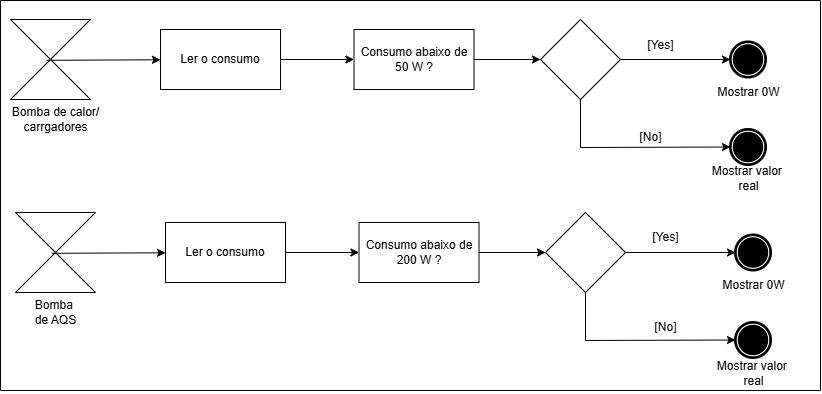
\includegraphics[width=\textwidth]{images/consumo_2.png}
    \caption{Diagrama de decisão bombas/carregadores}
    \label{fig:consumo_2.png}
\end{figure}

Encaixar todas as cards e entidades na main dashboard, foi também uma dificuldade, pois tivemos que encontrar o tamanho perfeito para cada, encaixando tudo na perfeição.
Também foi necessário criar um template sensor para somar os três valores de produção solar — \textit{PV1 Master}, \textit{PV2 Master} e \textit{PV1 Slave} — de forma a calcular a produção total proveniente dos painéis fotovoltaicos.\\
Adicionalmente, foi criado um sensor para o cálculo do consumo total da habitação, combinando a energia proveniente da produção solar, da rede elétrica (grid) e da bateria. No entanto, foram implementadas condições lógicas para garantir que apenas os fluxos de saída (exportação) do \textit{grid} e da bateria são considerados. Ou seja, se algum desses sistemas estiver a importar energia (ou seja, a consumir), esse valor é ignorado no cálculo do consumo total, garantindo uma leitura mais precisa e representativa da energia efetivamente utilizada na casa.\\
Adicionalmente, foi criado um botão de exportação energética com base num sensor personalizado (\textit{exportacao\_status}). Este sensor analisa o valor de potência da rede (\textit{sensor.rede\_power}) e, consoante o nível de exportação de energia para a rede (valores negativos), classifica a situação em quatro estados: \textit{ultra}, \textit{high}, \textit{medium} e \textit{low}.
Cada estado é representado visualmente através de um cartão interativo (\textit{custom:button-card}), com cores e ícones distintos que indicam se há excesso de produção solar, produção parcial ou dependência da rede elétrica. Esta abordagem permite ao utilizador identificar rapidamente o estado de exportação solar da habitação e tomar decisões informadas sobre o uso energético em tempo real. A Figura~\ref{fig:Saldo_Botao_Energetico_diagrama.drawio_2.png} ilustra o processo de decisão associado ao botão de exportação energética, com base nos níveis de potência exportada para a rede e respetiva codificação por cores.

\begin{figure}[H]
    \centering
    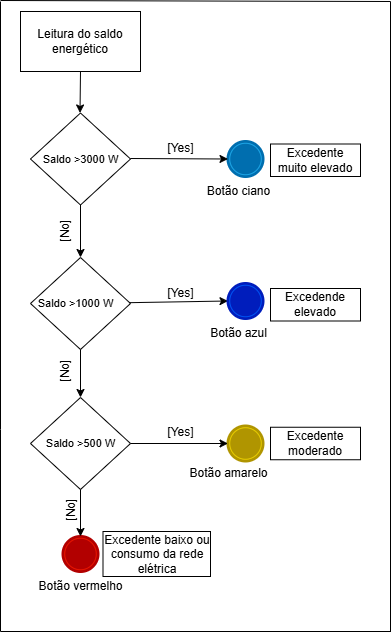
\includegraphics[height=0.4\textheight]{images/Saldo_Botao_Energetico_diagrama.drawio_2.png}
    \caption{Diagrama de decisão - Saldo energético}
    \label{fig:Saldo_Botao_Energetico_diagrama.drawio_2.png}
\end{figure}

\section{Dashboards produzidos}

\subsection{Dashboard Principal}

\begin{figure}[H]
    \centering
    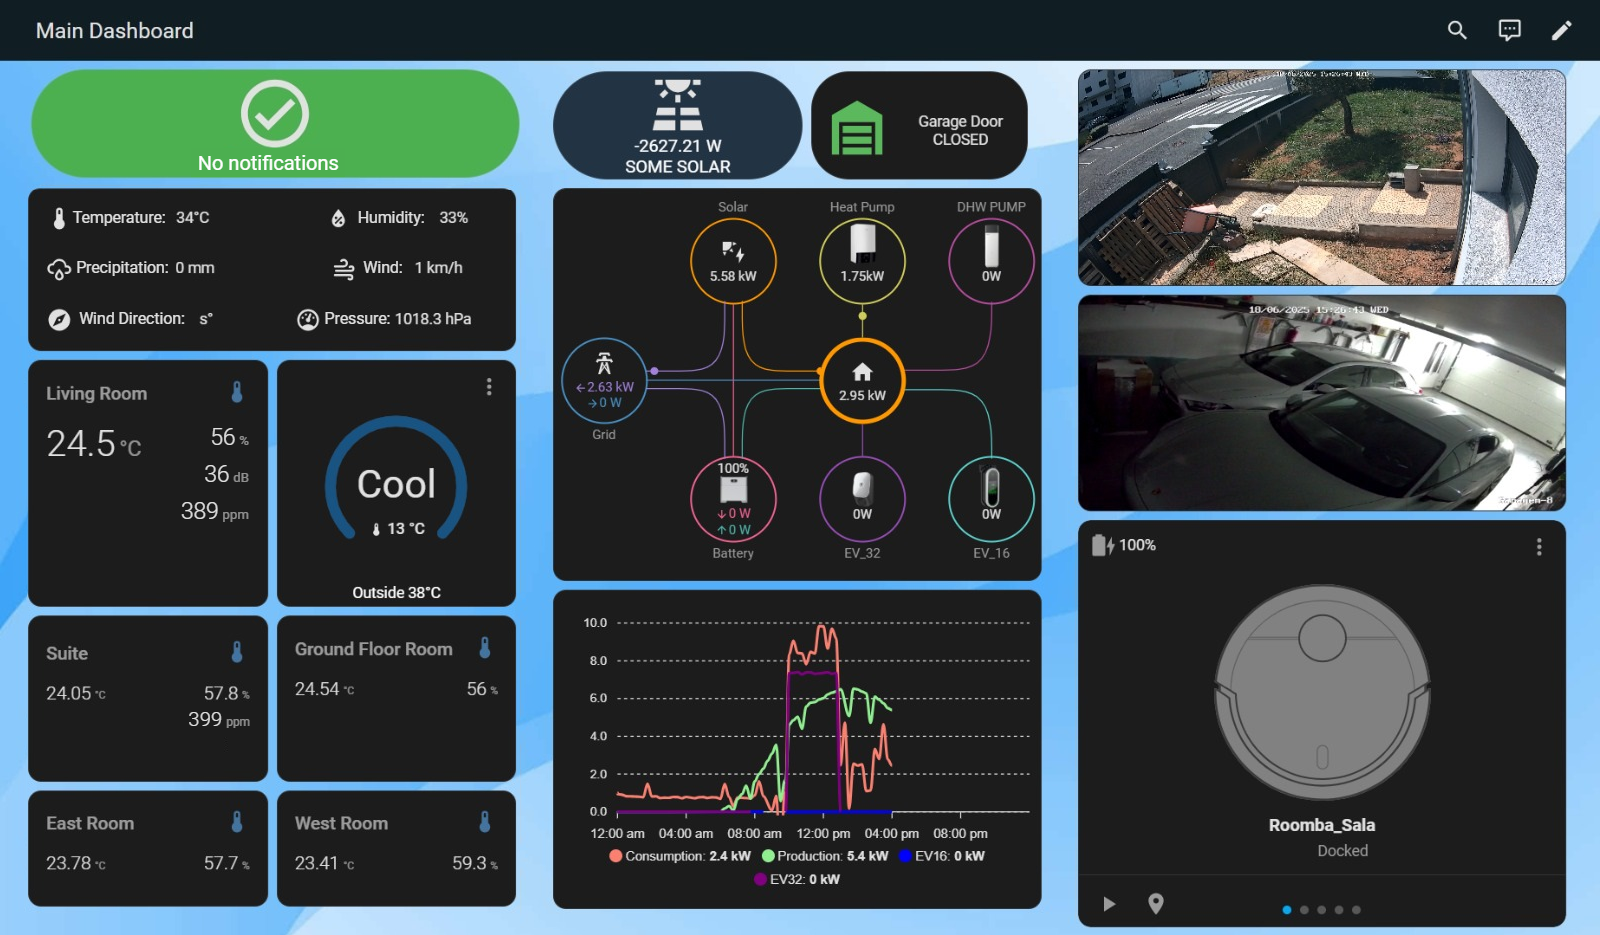
\includegraphics[width=\textwidth]{images/principal.png}
    \caption{Dashboard Principal}
    \label{fig:principal.png}
\end{figure}

A dashboard principal, chamada de \textit{Main Dashboard}, foi concebida para ser o painel principal do \gls{HA}, permitindo uma visão abrangente e imediata do estado geral da casa. Como podemos verificar na Figura~\ref{fig:principal.png}, a dashboard está dividida em três áreas distintas: a área da esquerda é dedicada ao conforto e ao ambiente, a zona central foca-se na parte energética e a área direita está orientada essencialmente à segurança. Esta organização permite uma fácil e rápida leitura da informação mais relevante da casa.

De seguida, serão explorados e explicados em detalhe os principais componentes da dashboard principal, com destaque para as integrações realizadas, os sensores utilizados, os valores apresentados em tempo real, o seu significado e as soluções adotadas para representar a informação de forma clara e funcional.




\subsubsection{Botão Notificações}

\begin{figure}[H]
    \centering
    
\includegraphics[width=0.6\textwidth]{images/botao_notificacoes.png}
    \caption{Botão Notificações}
    \label{fig:botao_notificacoes.png}
\end{figure}

O botão de notificações é uma funcionalidade essencial para garantir uma resposta rápida a eventos importantes na casa. Como ilustrado na Figura~\ref{fig:botao_notificacoes.png}, este botão assume uma aparência verde com a indicação \textnormal{"No notifications"} quando não há notificações ativas. Sempre que ocorre um evento relevante, como a abertura do portão da garagem, início de precipitação, deteção de níveis elevados de CO\textsubscript{2} (acima de 1000 ppm), ruído elevado (acima de 60 dB) ou o início de funcionamento de um robô aspirador, é gerado automaticamente um alerta visual.


\begin{table}[H]
\centering
\resizebox{!}{7.3cm}{
\rowcolors{2}{gray!10}{white}
\begin{tabularx}{\textwidth}{|p{6cm}|X|p{3cm}|}
\hline
\textbf{Condição} & \textbf{Entidade} & \textbf{Notificação} \\
\hline

Portão abriu & switch.portao\_garagem & Open gate \\

\% chuva > 0.1\%  & sensor.netatmo\_1piso\_rain\_gauge \_precipitation & Rain \\

CO2 acima de 1000  & sensor.netatmo\_1piso\_carbon \_dioxide & High CO2 \\

Noise acima de 60  & sensor.netatmo\_1piso\_noise & High Noise \\

Robo roomba da sala a limpar  & vacuum.roomba\_sala & Robot cleaning \\

Robo braava da sala a limpar  & vacuum.braava\_sala & Robot cleaning \\

Robo roomba piso a limpar  & vacuum.roomba\_piso & Robot cleaning \\

Robo roomba do bunker a limpar  & vacuum.roomba\_bunker & Robot cleaning \\

Robo roomba da cave a limpar  & vacuum.roomba\_cave & Robot cleaning \\

Bomba de calor ligou & sensor.bomba\_calor\_filtered\_power & Heat pump connected\\

Bomba de AQS ligou & sensor.bomba\_aqs\_filtered \_power & DHW pump connected\\

Vento forte & sensor.netatmo\_1piso\_anemometer \_wind\_speed &  Strong wind \\

Temperatura exterior abaixo de 0ºC & sensor.netatmo\_1piso\_netatmo \_exterior\_temperature & Negative temperature\\

Humidade exterior abaixo de 30\% & sensor.netatmo\_1piso\_netatmo \_exterior\_humidity & Negative humidity \\

Humidade exterior acima de 85\% & sensor.netatmo\_1piso\_netatmo \_exterior\_humidity & High humidity \\

Sem alertas  &  & No notifications \\

\hline
\end{tabularx}
}
\caption{Notificações, segundo condição.}
\end{table}

\subsubsection{Sensores Exteriores}

\begin{figure}[H]
    \centering
    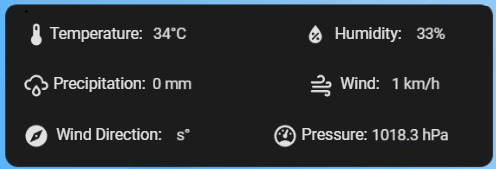
\includegraphics[width=0.6\textwidth]{images/sensores_exteriores.png}
    \caption{Sensores Exteriores}
    \label{fig:sensores_exteriores.png}
\end{figure}

A secção dos sensores exteriores (Figura~\ref{fig:sensores_exteriores.png}) fornece informação ambiental proveniente de sensores instalados no exterior da habitação. Os dados visíveis na dashboard incluem:

\begin{table}[H]
\centering
\begin{tabular}{|l|c|}
\hline
\textbf{Parâmetro}             & \textbf{Valor}       \\
\hline
Temperatura                   & 34 ºC                \\
Humidade                      & 33 \%                \\
Precipitação                  & 0 mm                 \\
Velocidade do vento           & 1 km/h               \\
Direção do vento              & Sul (S)              \\
Pressão atmosférica           & 1018.3 hPa           \\
\hline
\end{tabular}
\caption{Informações dos sensores exteriores.}
\end{table}

Estas informações são cruciais tanto para conforto como para automações, por exemplo, ajustar a climatização ou fechar estores em caso de aumento de temperatura ou vento forte.

\newpage

\subsubsection{Sensores Interiores}

\begin{figure}[H]
    \centering
    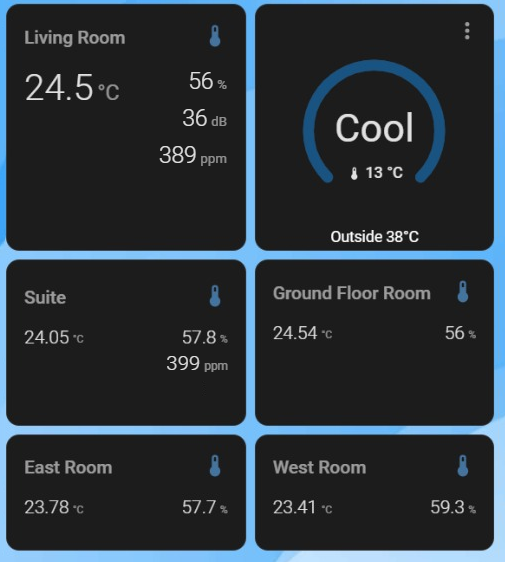
\includegraphics[width=0.6\textwidth]{images/sensores_interiores.png}
    \caption{Sensores Interiores}
    \label{fig:sensores_interiores.png}
\end{figure}

Os sensores interiores da Figura~\ref{fig:sensores_interiores.png} monitorizam temperatura, humidade, ruído e concentração de CO\textsubscript{2} em diferentes divisões da casa. Os dados disponíveis são os seguintes:

\begin{table}[H]
\centering
\begin{tabular}{|l|c|c|c|c|}
\hline
\textbf{Divisão} & \textbf{Temperatura} & \textbf{Humidade} & \textbf{Ruído} & \textbf{PPM} \\
\hline
Sala de Estar & 24.5 ºC & 56 \% & 36 dB & 389 ppm \\
Suite & 24.05 ºC & 57.8 \% & -- & 399 ppm \\
Quarto Rés-do-chão & 24.54 ºC & 56 \% & -- & -- \\
Quarto Este & 23.78 ºC & 57.7 \% & -- & -- \\
Quarto Oeste & 23.41 ºC & 59.3 \% & -- & -- \\
\hline
\end{tabular}
\caption{Dados dos sensores interiores por divisão}
\label{tab:sensores_interiores}
\end{table}

Na zona da sala, além da temperatura e humidade, é apresentado o estado atual do ar condicionado, indicando que está a arrefecer (\textit{Cool}) para atingir a temperatura da água definida de \textbf{13 ºC} e também a temperatura exterior de \textbf{38 ºC}.

\subsubsection{Botões Energia}

\begin{figure}[H]
    \centering
    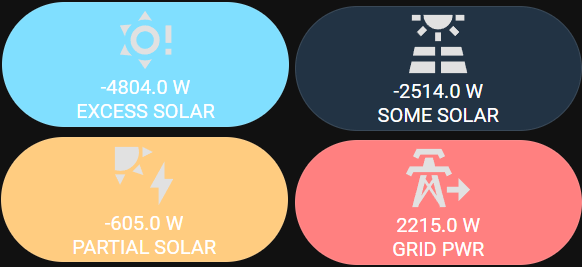
\includegraphics[width=0.6\textwidth]{botoes_energia.png}
    \caption{Botões Energia}
    \label{fig:botoes_energia.png}
\end{figure}

O botão da Figura~\ref{fig:botoes_energia.png}, fornece uma representação visual e imediata do \textbf{saldo energético} da casa, isto é, a diferença entre a energia produzida, pelos painéis solares e a consumida pela casa e seus dispositivos. A principal funcionalidade deste botão é alertar o utilizador para o estado energético com base numa escala de cores:

\begin{table}[H]
\centering
\begin{tabular}{|l|l|l|}
\hline
\textbf{Cor} & \textbf{Condição} & \textbf{Texto Botão} \\
\hline
\textcolor{cyan}{Ciano}   & Exportação superior a 3000~W & EXCESS SOLAR \\
\textcolor{blue}{Azul}    & Exportação superior a 1000~W & SOME SOLAR\\
\textcolor{yellow}{Amarelo} & Exportação superior a 500~W & PARTIAL SOLAR\\
\textcolor{red}{Vermelho} & Exportação inferior a 500~W ou consumo da rede elétrica & GRID PWR\\
\hline
\end{tabular}
\caption{Detalhe do botão de exportação de energia.}
\end{table}


\subsubsection{Botão Garagem}

\begin{figure}[H]
    \centering
    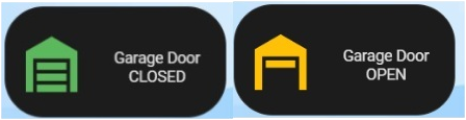
\includegraphics[width=0.6\textwidth]{botao_garagem.png}
    \caption{Botão Garagem.}
    \label{fig:botao_garagem.png}
\end{figure}

Na Figura~\ref{fig:botao_garagem.png}, temos um botão que permite controlar o \textbf{portão da garagem}, apresentando simultaneamente o seu estado atual e permitindo interagir com o sistema. A cor do botão indica o estado:

\begin{table}[H]
\centering
\begin{tabular}{|c|l|}
\hline
\textbf{Cor} & \textbf{Estado do Portão} \\
\hline
\textcolor{green}{Verde} & Portão fechado \\
\textcolor{orange}{Laranja} & Portão aberto \\
\hline
\end{tabular}
\caption{Detalhe do botão do portão.}
\label{tab:estado_portao}
\end{table}


Além da indicação visual, o botão permite também \textbf{abrir ou fechar o portão} ao ser pressionado por mais de 2 segundos, evitando assim ativações acidentais com toques breves.

\subsubsection{Diagrama Energia}

\begin{figure}[H]
    \centering
    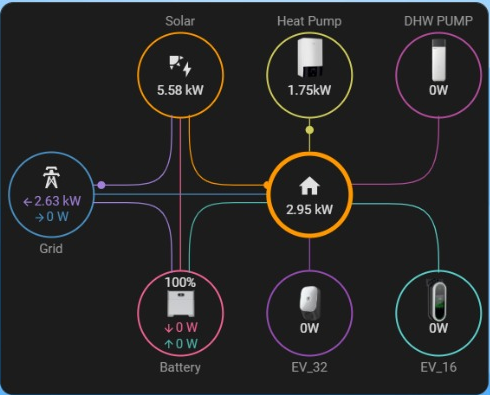
\includegraphics[width=0.6\textwidth]{images/diagrama_energia.png}
    \caption{Diagrama Energia}
    \label{fig:diagrama_energia.png}
\end{figure}

O diagrama energético apresentado na Figura.~\ref{fig:diagrama_energia.png} fornece uma representação gráfica em tempo real dos fluxos de energia entre os principais elementos do sistema energético da casa. É de fácil e rápida visualização, permitindo ao utilizador identificar rapidamente os consumos, produções e fluxos bidirecionais.

Os painéis solares encontram-se a produzir \textbf{5.58 kW}, valor superior ao consumo da habitação, que se encontra nos \textbf{2.95 kW}. A totalidade do consumo está a ser suprida pela produção solar, e o excedente de \textbf{2.63 kW} está a ser injetado na rede elétrica. A bateria encontra-se totalmente carregada (\textbf{100\%}) e, neste momento, não está nem a descarregar nem a carregar (\textbf{0 W}). Relativamente aos consumos específicos:

\begin{table}[H]
\centering
\begin{tabular}{|l|c|}
\hline
\textbf{Equipamento} & \textbf{Consumo} \\
\hline
Bomba de Calor (Heat Pump) & \textbf{1.75 kW}  \\
Bomba de Água Quente (DHW Pump) & \textbf{0 W} \\
Carregador EV\_32 & \textbf{0 W} \\
Carregador EV\_16 & \textbf{0 W} \\
\hline
\end{tabular}
\caption{Consumo dos principais equipamentos}
\label{tab:consumos_equipamentos}
\end{table}

Esta representação intuitiva permite um acompanhamento imediato do comportamento energético da habitação, facilitando ações rápidas de otimização ou diagnósticos de consumo e produção.

\subsubsection{Gráfico Energético}
\begin{figure}[H]
    \centering
    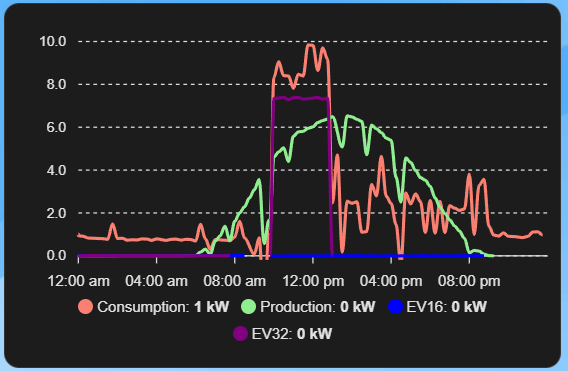
\includegraphics[width=\textwidth]{images/grafico_energia.png}
    \caption{Gráfico Energético}
    \label{fig:grafico_energia.png}
\end{figure}

O gráfico energético da Figura~\ref{fig:grafico_energia.png} apresenta a evolução do \textbf{consumo}, \textbf{produção} e utilização dos \textbf{carregadores elétricos} ao longo das últimas 24 horas. As curvas no gráfico têm as seguintes cores:

\begin{table}[H]
\centering
\begin{tabular}{|c|l|}
\hline
\textbf{Cor} & \textbf{Significado} \\
\hline
\textcolor{orange}{Laranja} & Consumo da casa \\
\textcolor{green}{Verde} & Produção fotovoltaica \\
\textcolor{violet}{Roxo} & Carregador EV\_32 \\
\textcolor{blue}{Azul} & Carregador EV\_16 \\
\hline
\end{tabular}
\caption{Detalhe do gráfico energético.}
\label{tab:cores_consumo_producao}
\end{table}

\vspace{1em}

\begin{flushleft}
\vspace{-\baselineskip} % remove espaço extra que o LaTeX pode deixar
\begin{itemize}[itemsep=0pt, parsep=0pt, partopsep=0pt, topsep=0pt, leftmargin=*]
  \item O consumo da casa apresenta picos acentuados entre as 10h00 e as 13h00, e variações moderadas no restante do dia.
  \item A produção fotovoltaica inicia-se por volta das 06h30, atinge o pico por volta do meio-dia (acima dos \textbf{6 kW}) e mantém-se estável até às 15h00, diminuindo depois gradualmente.
  \item O carregador EV\_32 esteve ativo apenas entre as 10h00 e as 14h00, coincidindo com o período de maior produção solar.
  \item O carregador EV\_16 continua sem registos de utilização significativos.
\end{itemize}
\end{flushleft}




Este gráfico permite identificar claramente os períodos de maior produção e consumo energético, contribuindo para uma gestão otimizada do autoconsumo e do carregamento de veículos elétricos com base no excedente solar disponível.

\subsubsection{Câmaras}

\begin{figure}[H]
    \centering
    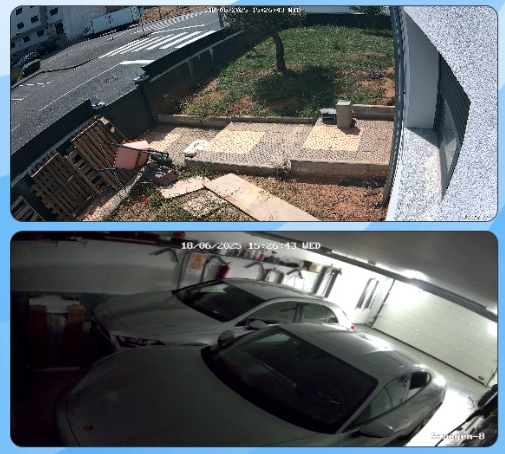
\includegraphics[width=0.6\textwidth]{images/camaras_main.png}
    \caption{Câmaras}
    \label{fig:camaras_main.png}
\end{figure}

A secção de segurança da dashboard inclui uma visualização em tempo real de duas câmaras de videovigilância, conforme mostrado na Figura~\ref{fig:camaras_main.png}. A primeira câmara está direcionada para a entrada exterior da habitação, permitindo monitorizar acessos e movimentos. A segunda câmara está posicionada na garagem, garantindo a segurança dos veículos e deteção de movimentos suspeitos. A integração destas câmaras oferece maior controlo e tranquilidade ao utilizador, permitindo uma resposta rápida em caso de atividade anómala.

\subsubsection{Aspiradores}

\begin{figure}[H]
    \centering
    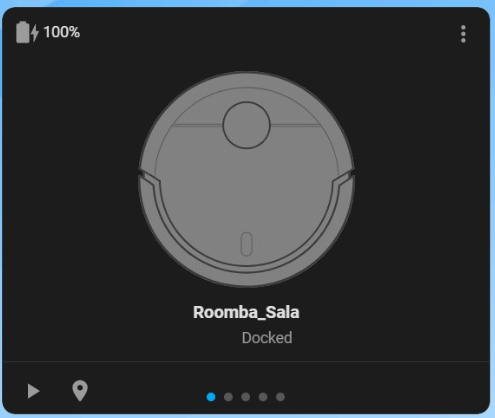
\includegraphics[width=0.6\textwidth]{images/aspiradores_main.png}
    \caption{Aspiradores}
    \label{fig:aspiradores_main.png}
\end{figure}

Na parte inferior direita da dashboard encontra-se um cartão interativo (Figura ~\ref{fig:aspiradores_main.png}) dedicado à gestão dos aspiradores robóticos. Utilizando o cartão \textit{swipe card}, é possível alternar rapidamente entre os diferentes aspiradores instalados em várias divisões da casa (5 no total). Cada cartão exibe o estado atual do dispositivo (por exemplo, “\textit{Docked}”), a bateria (por exemplo, 100\%) e permite o controlo direto de ações como iniciar ou pausar a limpeza, ou enviar o robô de volta para a base.

\newpage

\subsection{Dashboard Energia}

\begin{figure}[H]
    \centering
    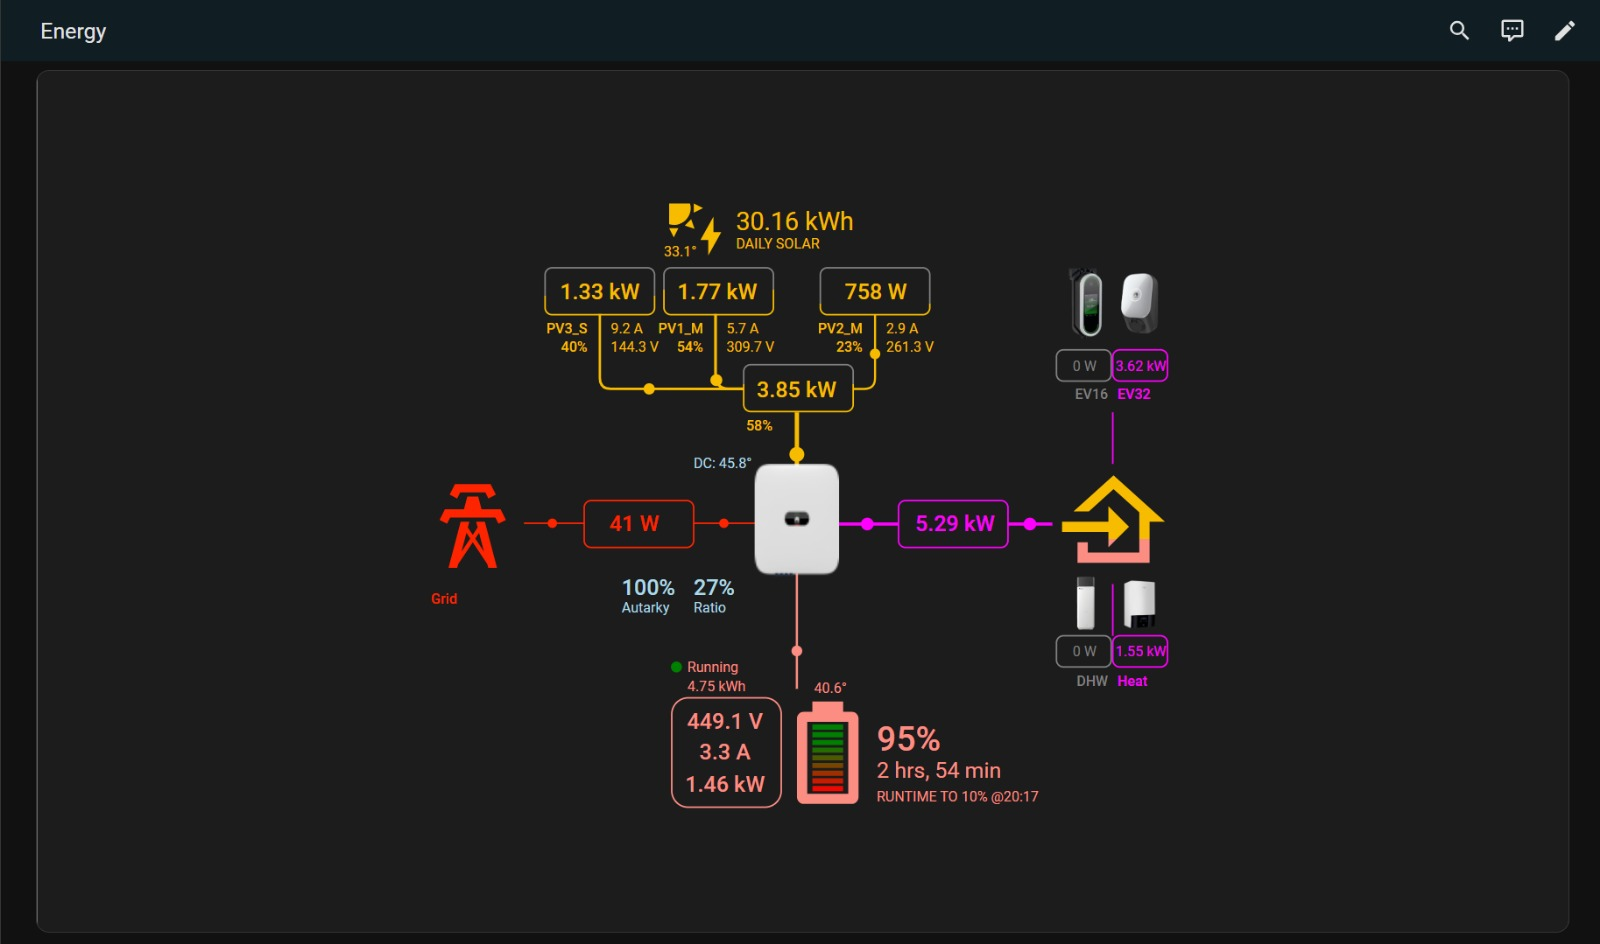
\includegraphics[width=\textwidth]{energia.png}
    \caption{Dashboard Energia}
    \label{fig:energia.png}
\end{figure}

Como mostrado na Figura.~\ref{fig:energia.png}, esta dashboard apresenta uma visão detalhada e em tempo real do sistema energético da habitação. No topo, observa-se a produção solar diária acumulada, com um total de \textbf{30,16~kWh}. Esta energia é proveniente de três \textit{strings} fotovoltaicas individuais (PV3\_S, PV1\_M e PV2\_M), que, no momento, produziam \textbf{1,33~kW}, \textbf{1,77~kW} e \textbf{758~W}, respetivamente, totalizando uma produção atual de \textbf{3,85~kW}.

Ao centro, encontra-se o inversor \textit{Huawei}, que agrega a produção solar e gere a distribuição da energia. A casa consome, neste momento, \textbf{5,29~kW}, com destaque para o carregamento do veículo \textit{EV32}, que consome \textbf{3,62~kW}, e para o sistema de aquecimento, responsável por \textbf{1,55~kW}. Os restantes dispositivos ligados à casa, nomeadamente o \textit{EV16} e o sistema de \textit{DHW} (águas quentes sanitárias), encontram-se em \textit{standby}, apresentando, por isso, um consumo de \textbf{0~W}. Este valor foi definido para simplificar a visualização da interface, considerando-se como \textit{standby} os seguintes critérios: consumos inferiores a \textbf{50~W} nos carregadores de veículos elétricos (\textit{EV}) e na bomba de \textit{AQS}, bem como consumos inferiores a \textbf{200~W} no sistema de bomba de calor. Nestes casos, o valor apresentado é \textbf{0~W}.

No lado esquerdo do diagrama, é visível a importação de energia da rede elétrica, com um valor de \textbf{41~W}. Isto indica que, apesar da produção solar, a energia gerada não é suficiente para suprir totalmente o consumo atual.

Na parte inferior, encontra-se o estado da bateria, que está com 95\% de carga e fornece \textbf{1,46~kW} para ajudar a suprir o consumo da casa. A estimativa de autonomia restante indica cerca de 2~horas e 54~minutos até atingir 10\% de carga, por volta das 20:17. A temperatura interna da bateria é de 40{,}6~ºC.

Este \textit{layout} dinâmico e intuitivo permite uma leitura clara dos fluxos energéticos entre os vários componentes: produção solar, rede elétrica, bateria, consumos da casa, consumo da bomba de calor e \textit{AQS}, e carregamento do veículo elétrico.

O uso do cartão \textit{"Picture Elements Card"} foi essencial para sobrepor ícones representativos dos dispositivos reais, tornando a visualização mais interativa e compreensível para o utilizador.

\subsection{Dashboard de aquecimento}

\begin{figure}[H]
    \centering
    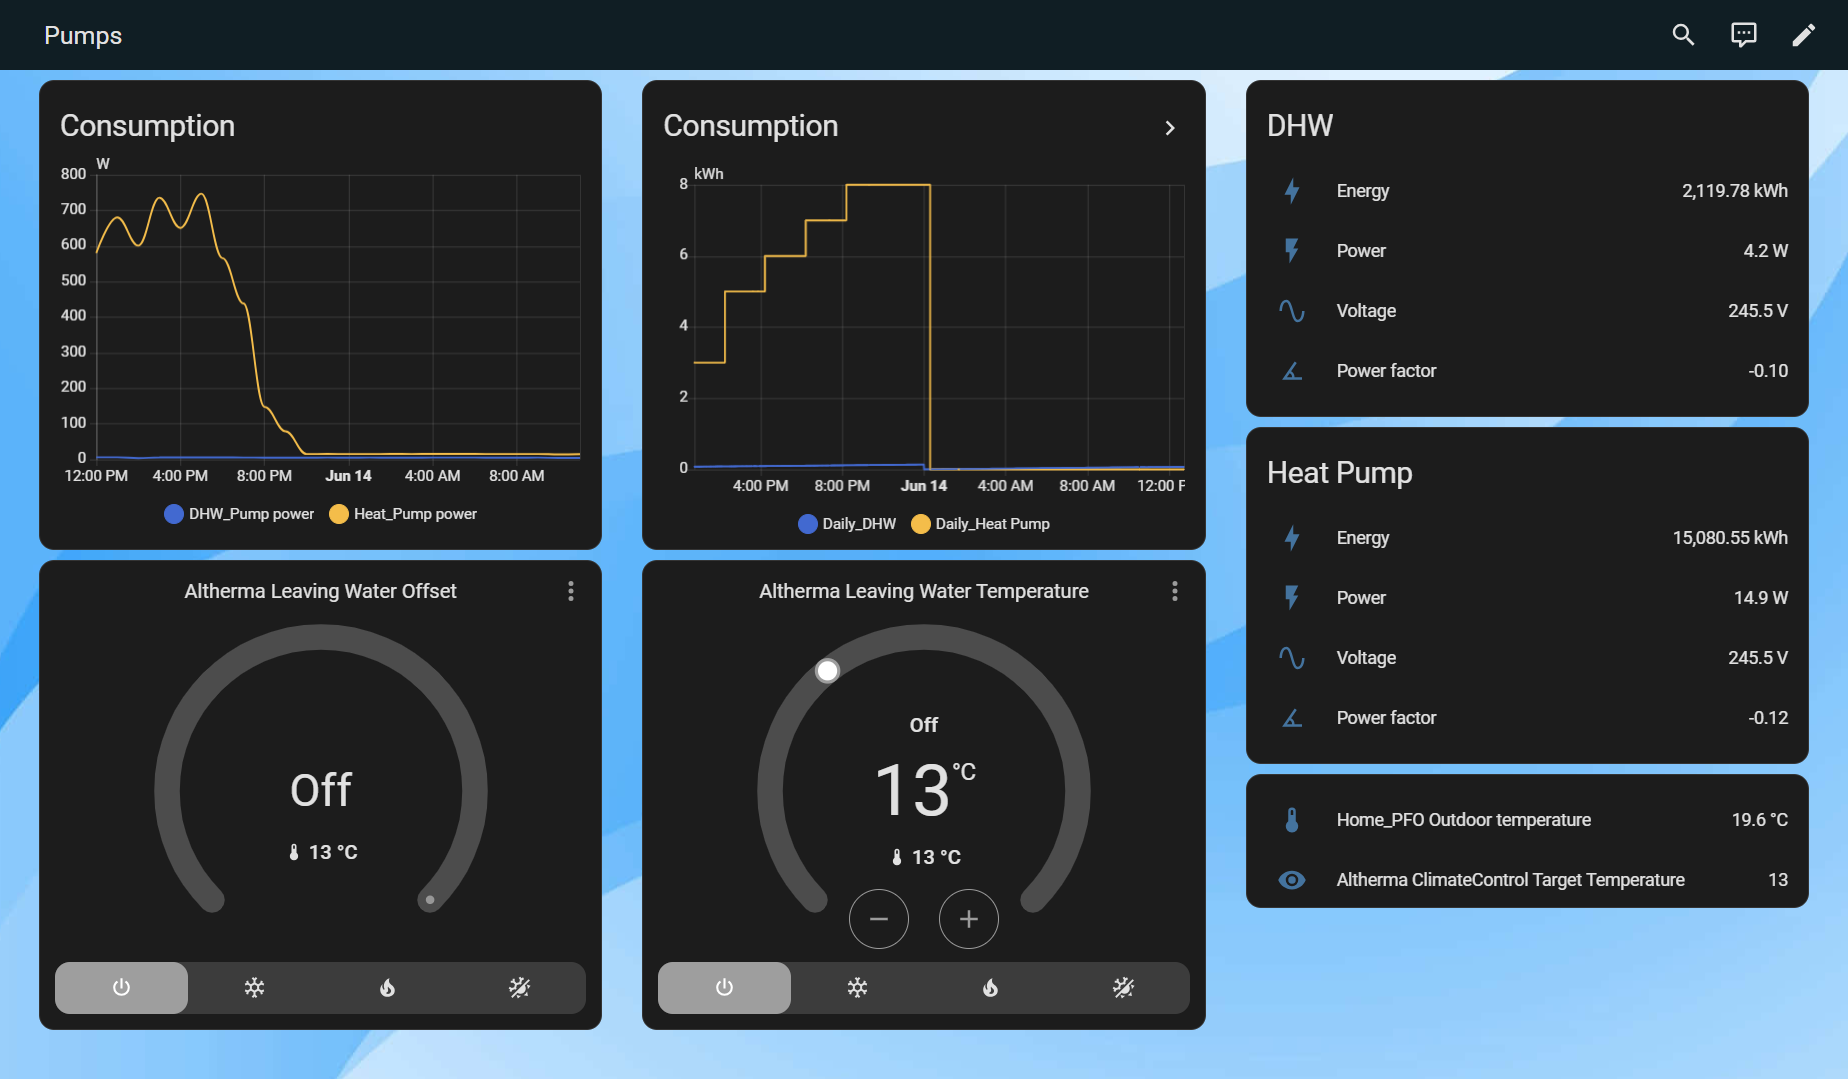
\includegraphics[width=\textwidth]{bombas.png}
    \caption{Dashboard Bombas}
    \label{fig:bombas.png}
\end{figure}

A interface apresentada na Figura~\ref{fig:bombas.png} fornece uma visão clara e organizada do sistema de aquecimento, com foco na bomba de calor \textit{Altherma} e na bomba de água quente sanitária (AQS). O dashboard está dividido em vários componentes principais:

\begin{itemize}
    \item \textbf{Gráficos de Consumo Diário e Potência}:
    \begin{itemize}
        \item \textbf{Consumo Diário da Bomba de Calor}: um gráfico complementar que reforça a análise do consumo diário de energia do sistema \textit{Altherma}.
        \item \textbf{Consumo Diário da Bomba AQS}: mostra o consumo diário da bomba de AQS, com um aumento constante ao longo do dia, ultrapassando os 8 kWh.
        \item \textbf{Potência da Bomba AQS}: mostra a potência da bomba de AQS, atingindo valores superiores a 500 W.
        \item \textbf{Potência da Bomba de Calor}: mostra a potência da bomba de calor.
    \end{itemize}
    
    \item \textbf{Controlo de Temperatura e Modo} (canto inferior esquerdo): Dois cartões de controlo permitem o ajuste direto da temperatura e do modo de funcionamento da bomba:
    \begin{itemize}
        \item \textbf{Aquecimento}: De momento desligado, OFF, e em modo \textit{Arrefecimento}, com a temperatura de saída da água definida para 13 ºC.
        \item \textbf{Arrefecimento}: também definido para 13 ºC, com o sistema a operar ativamente em modo de arrefecimento.
    \end{itemize}
    
    \item \textbf{Informações Adicionais} (direita): Apresenta métricas complementares do sistema, como o consumo de energia da bomba AQS (2110.11 kWh), potência (7.1 W), voltagem (241.6 V) e fator de potência (-0.17). Para a bomba de calor, o consumo de energia é de 15003.56 kWh, com um consumo atual de potência de 1132.9 W, voltagem de 241.6 V e fator de potência de -0.91. A temperatura exterior é de 14.41ºC, e a temperatura alvo da \textit{Altherma} está atualmente definida para 13ºC.
\end{itemize}

\newpage

\subsection{Dashboard Termostatos}

\begin{figure}[H]
    \centering
    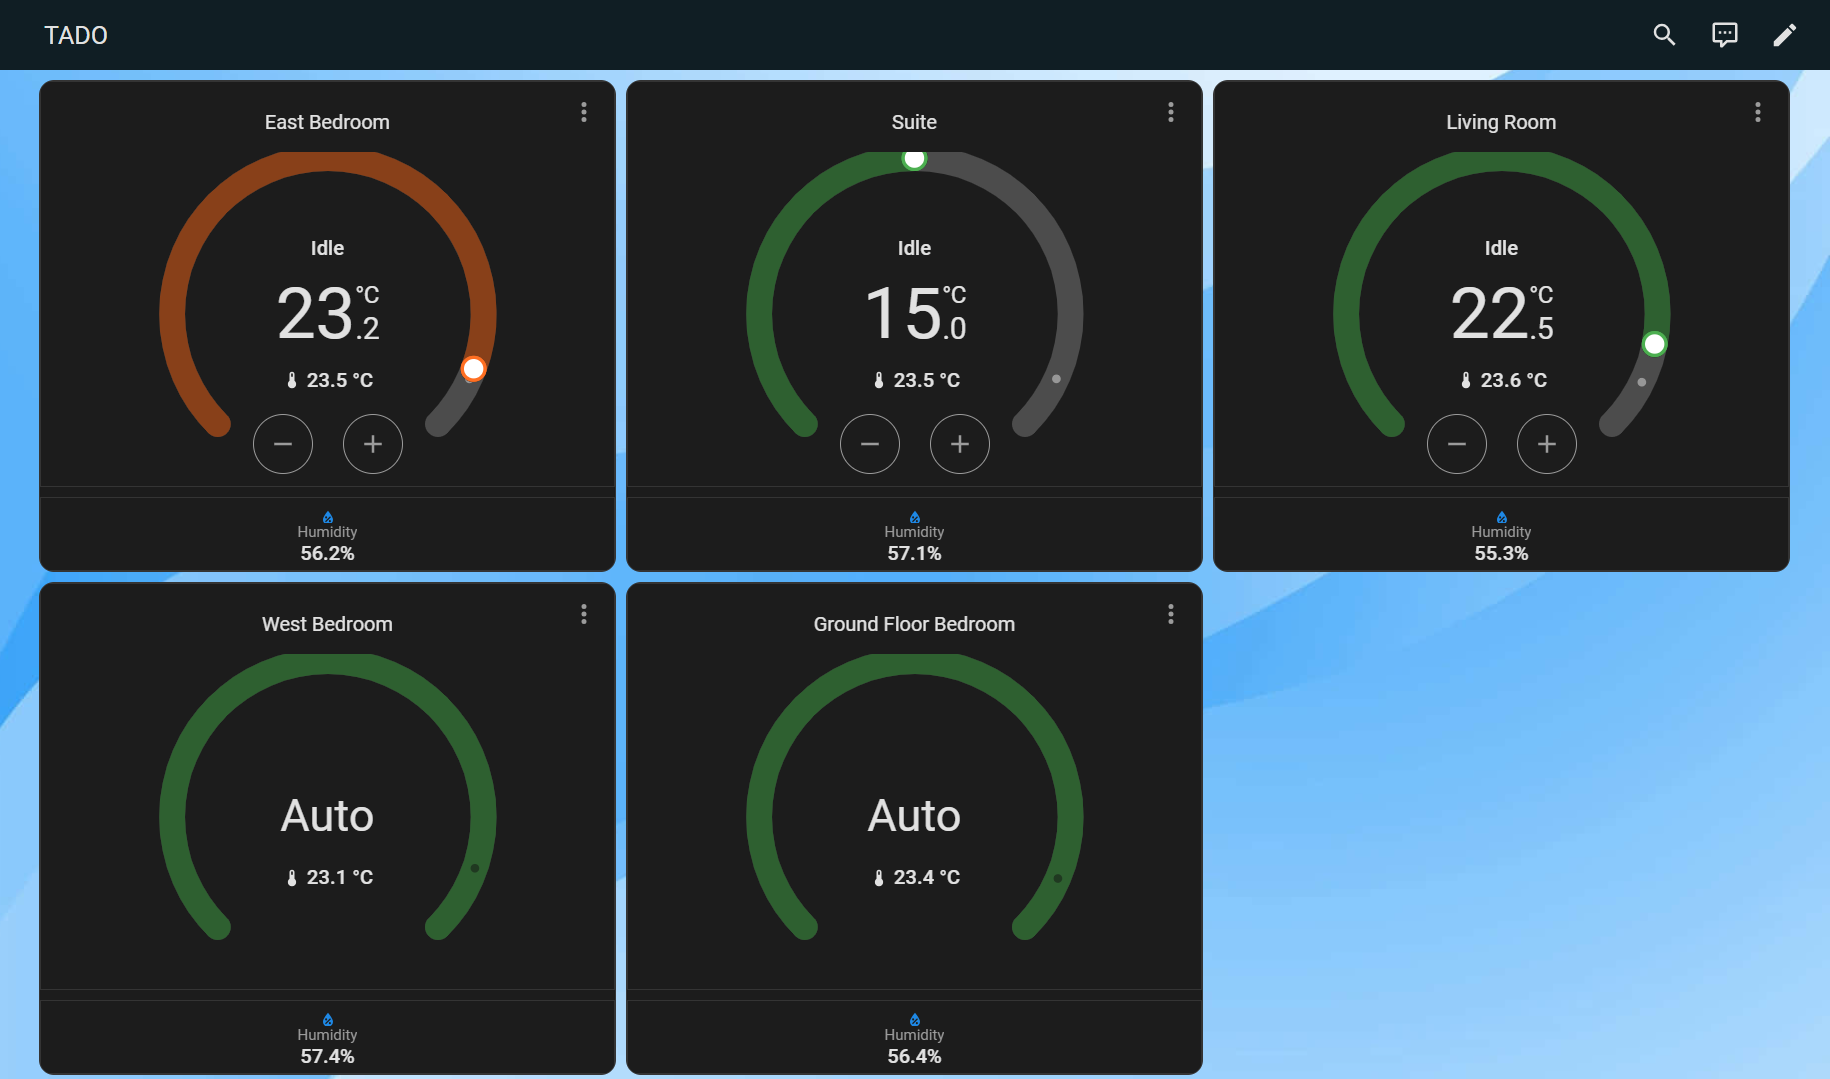
\includegraphics[width=\textwidth]{termostatos.png}
    \caption{Dashboard Termostatos}
    \label{fig:termostatos.png}
\end{figure}

A Figura~\ref{fig:termostatos.png} fornece uma visão abrangente do sistema de controlo climático interior, apresentando o estado atual dos termóstatos em várias divisões da casa. Cada cartão mostra a temperatura atual, a humidade relativa e o modo de funcionamento configurado (por exemplo, \textit{Auto} ou valor manual definido).

Segue-se um resumo dos dados apresentados:

\begin{itemize}
    \item \textbf{Quarto Este}: A temperatura atual é de 23,2ºC e o termóstato está definido manualmente para 23,1ºC. A divisão encontra-se inativa e a humidade é de 51,5\%.
    
    \item \textbf{Suite}: O termóstato está definido para uma temperatura alvo bastante inferior, 15,0ºC, enquanto a temperatura atual da divisão é de 23,4ºC, com uma humidade de 51,8\%. Isto sugere que está previsto arrefecimento, mas o sistema permanece inativo.
    
    \item \textbf{Sala de Estar}: A temperatura alvo é de 22,5ºC, com uma temperatura real de 23,6ºC e 50,1\% de humidade. O sistema encontra-se inativo, o que é expectável devido à pequena diferença entre a temperatura atual e a desejada.
\end{itemize}

Esta interface proporciona tanto visibilidade em tempo real como controlo sobre as condições térmicas de cada área da habitação. Promove a eficiência energética ao permitir ao utilizador adaptar o sistema de climatização apenas onde é necessário, e identificar divisões com temperaturas ou níveis de humidade inconsistentes.


\subsection{Dashboard Vigilância}

\begin{figure}[H]
    \centering
    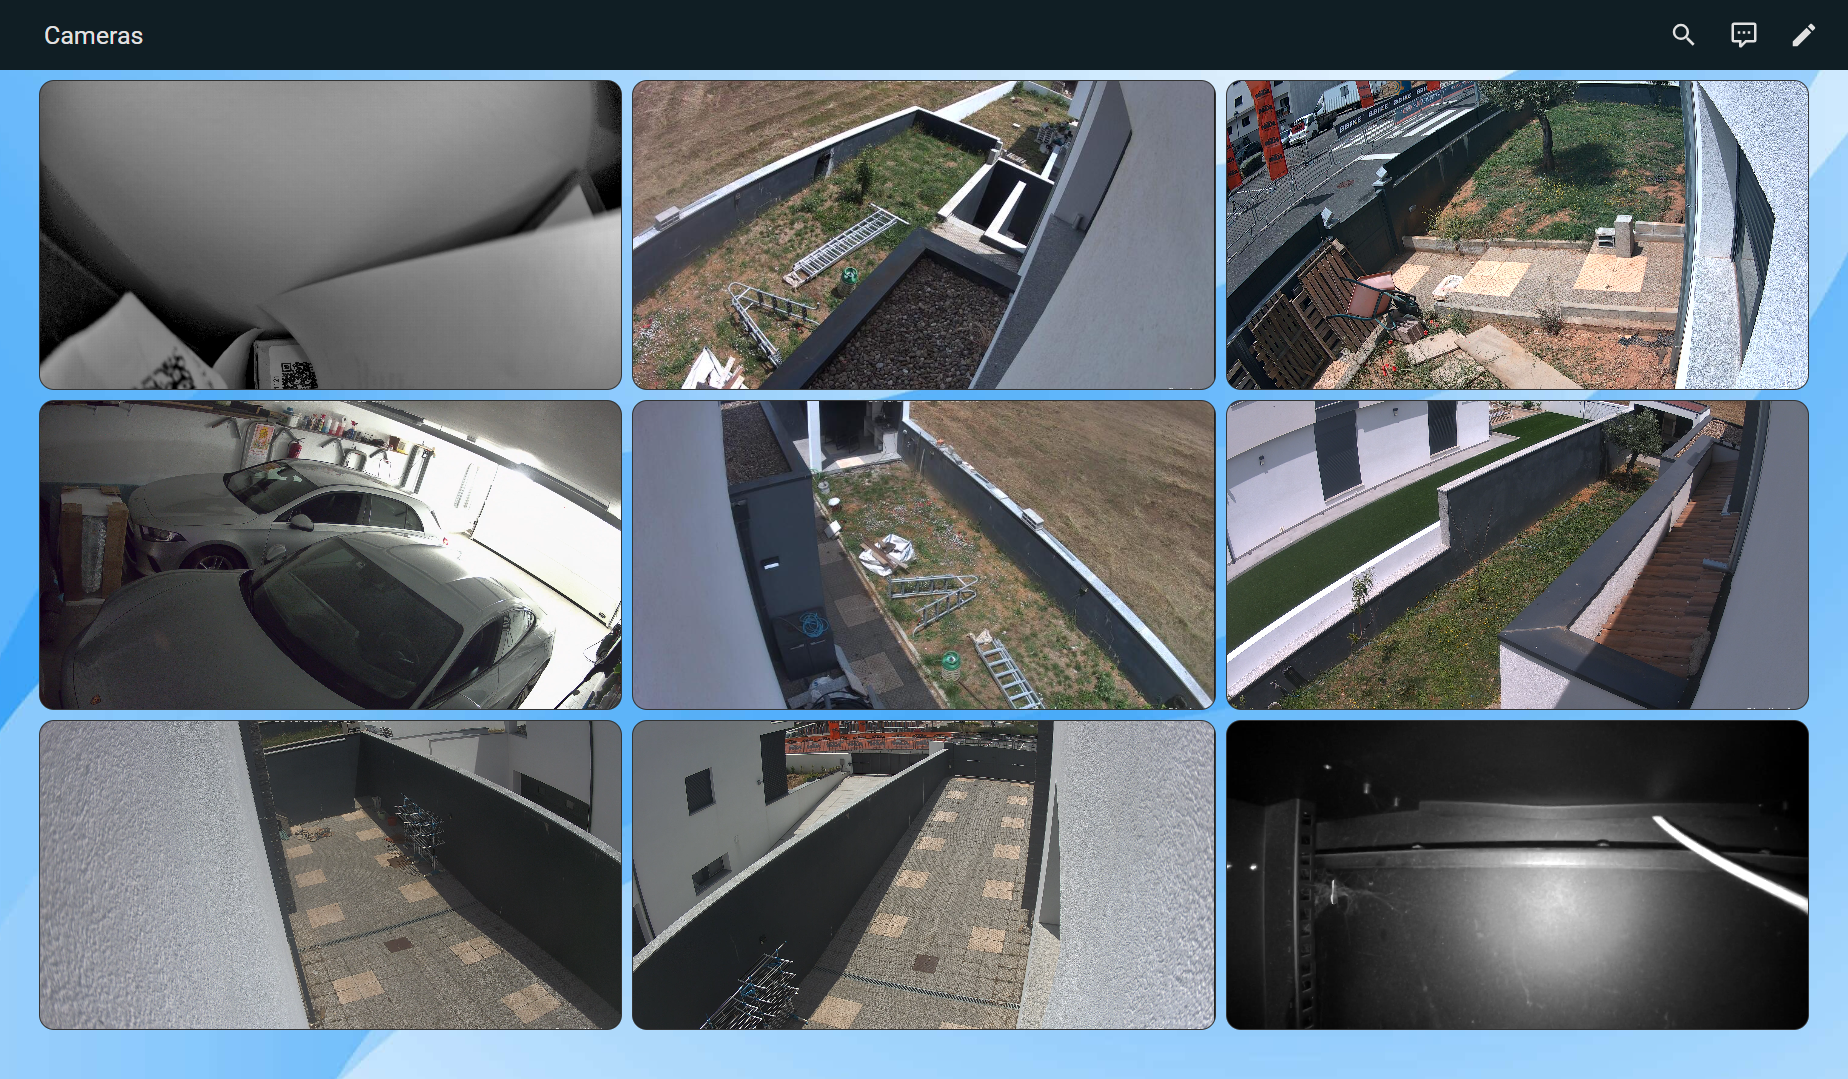
\includegraphics[width=\textwidth]{camaras.png}
    \caption{Dashboard Vigilância}
    \label{fig:camaras.png}
\end{figure}


Como mostrado na Figura~\ref{fig:camaras.png}, esta dashboard é inteiramente dedicada à monitorização em tempo real do sistema de videovigilância da propriedade. Apresenta uma grelha estruturada com nove transmissões de câmaras, cobrindo várias áreas exteriores. As câmaras captam diferentes perspetivas dos arredores, incluindo caminhos de acesso, paredes laterais e zonas do perímetro.

A imagem central na segunda linha mostra claramente o interior da garagem. É de notar que a transmissão da câmara no canto inferior direito corresponde a uma integração com a Netatmo, que fornece cobertura adicional com capacidades de deteção inteligente.

\subsection{Dashboard Estores}

\begin{figure}[H]
    \centering
    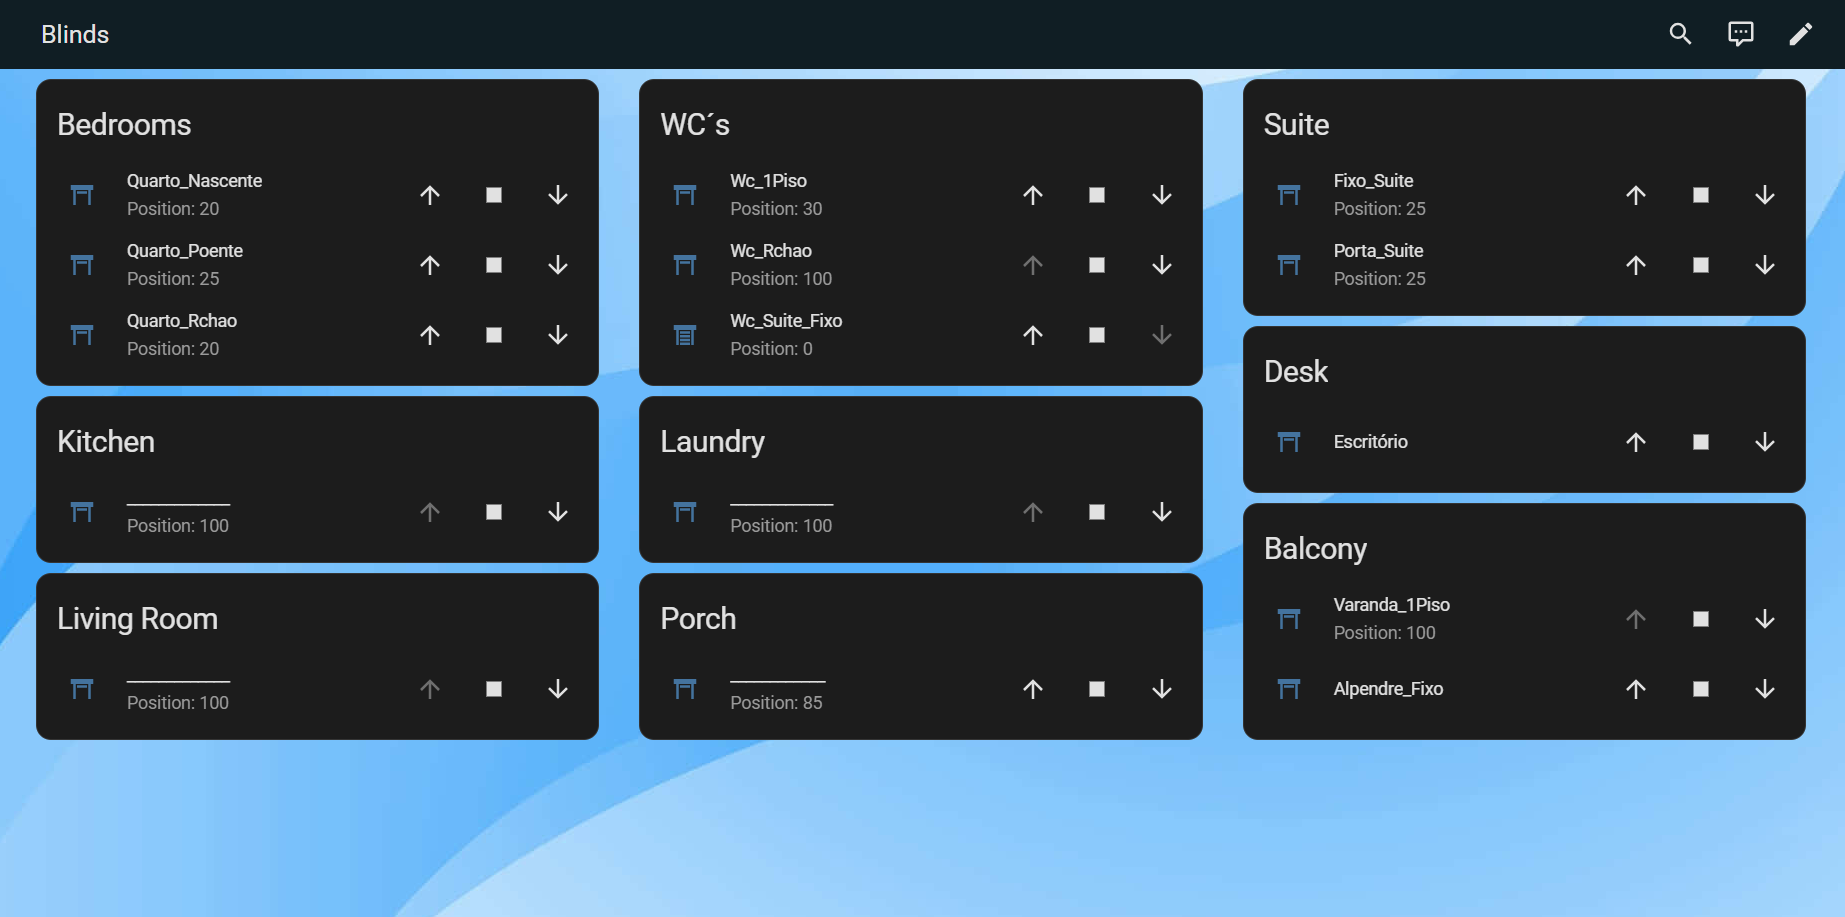
\includegraphics[width=\textwidth]{images/estores.png}
    \caption{Dashboard Estores}
    \label{fig: estores.png}
\end{figure}

Na Figura~\ref{fig: estores.png} é possível observar a dashboard dos estores com 3 botões cada:

\begin{itemize}
    \item \textbf{Seta para cima}: abre o estore.
    \item \textbf{Botão quadrado}: pára o estore na posição atual.
    \item \textbf{Seta para baixo}: fecha o estore.
\end{itemize}

As divisões com múltiplos estores (como a \textit{Suite} ou os \textit{Quartos}) apresentam cada dispositivo individualmente com o respetivo nome. O layout é responsivo e foi desenhado para permitir uma identificação visual rápida e controlo manual de todos os estores automatizados da habitação.

É ainda possível observar a sua posição, sendo "100\%" aberto e "0\%" fechado.

\newpage


\subsection{Dashboard Informação Ambiental}

\begin{figure}[H]
    \centering
    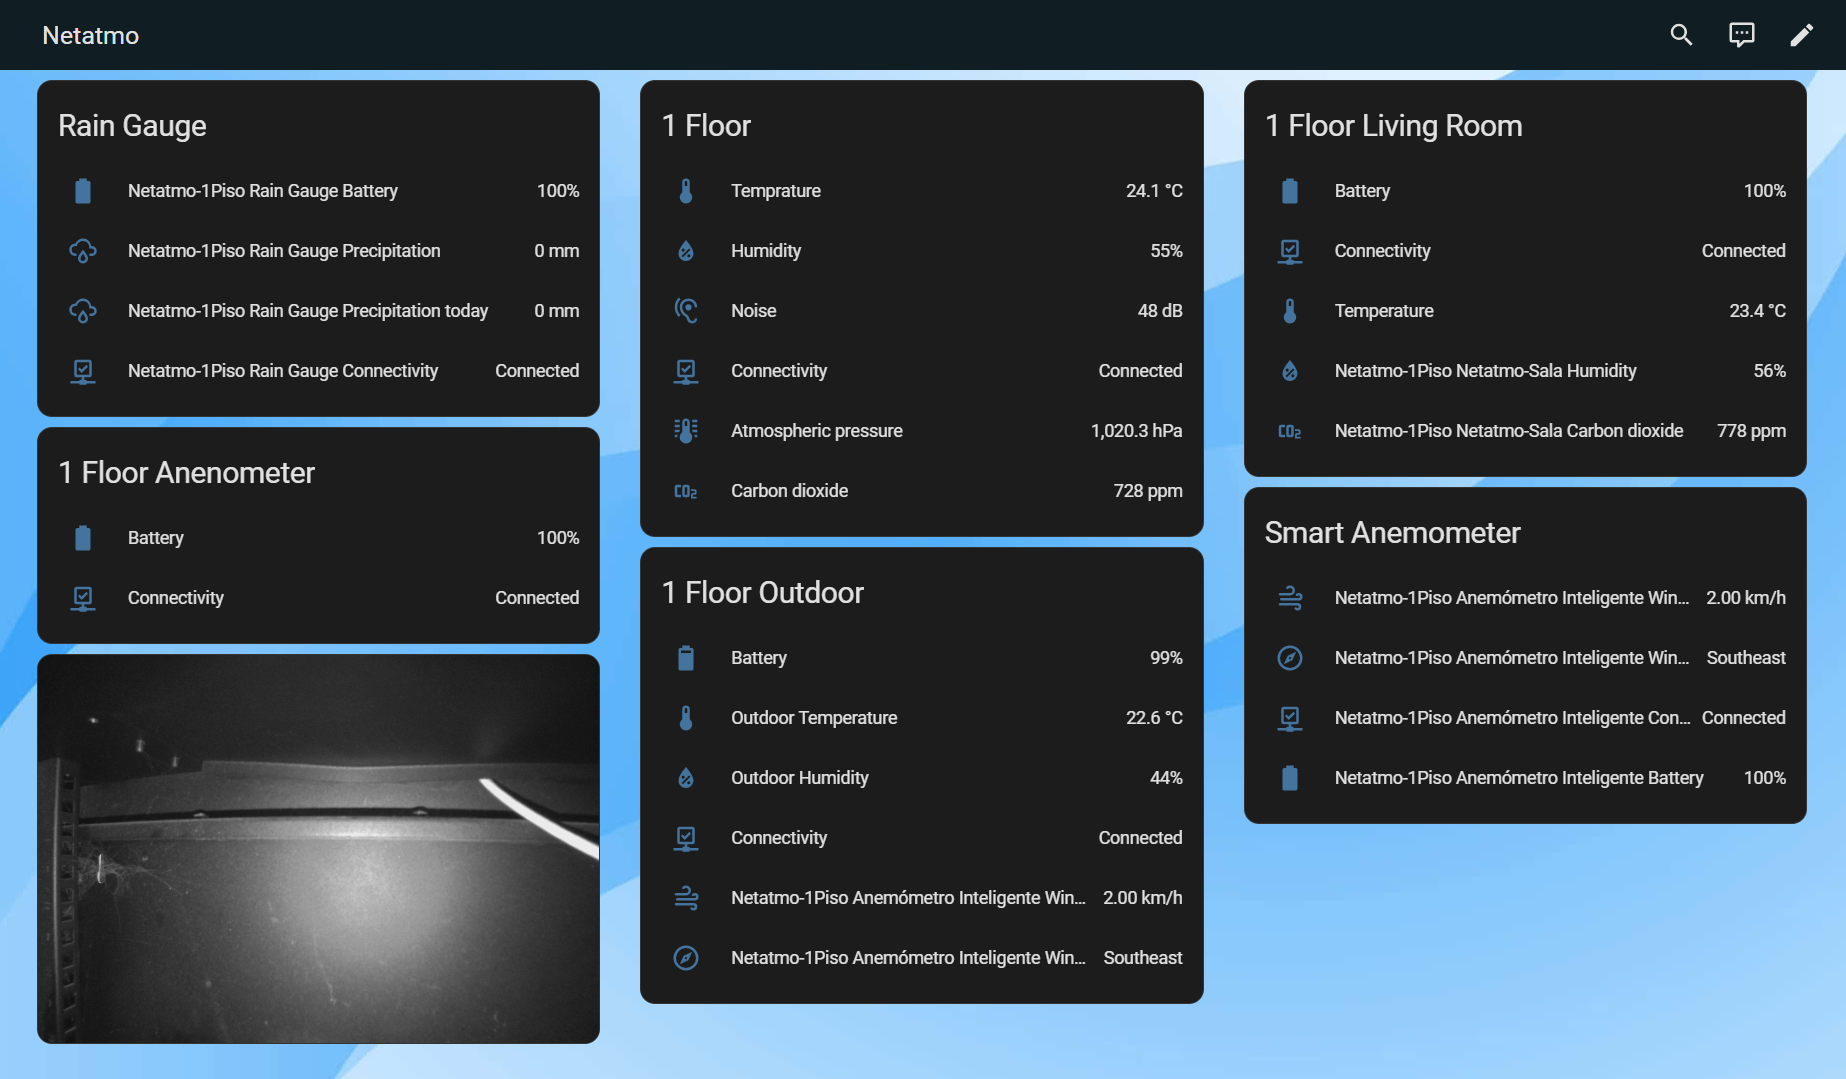
\includegraphics[width=\textwidth]{images/netatmo.png}
    \caption{Dashboard Informação Ambiental}
    \label{fig: netatmo.png}
\end{figure}

A Figura~\ref{fig: netatmo.png} apresenta o dashboard da informação ambiental, que fornece uma visão compacta e clara de vários sensores distribuídos pela casa. No canto inferior esquerdo, uma transmissão de câmara monitoriza a área física onde estão instalados alguns dos sensores.

O cartão \textnormal"1 Floor" (centro superior) exibe o módulo interior principal, localizado no primeiro andar, com leituras de temperatura (24,1ºC), humidade (55\%), ruído (48 dB), pressão atmosférica (1020,3 hPa) e CO2 (728 ppm), com conectividade ativa.

Na secção “1 Floor Living Room”, o módulo apresenta uma temperatura de 23,4ºC, humidade de 56\% e concentração de CO2 de 778 ppm, também com ligação estável. O módulo exterior, indicado em “1 Floor Outdoor”, reporta uma temperatura de 22,6ºC e humidade de 44\%, com bateria a 99\% e conectividade ativa.

O módulo “Rain Gauge” regista precipitação atual e diária como 0 mm, com ligação estável e bateria a 100\%. Já o módulo "Smart Anemometer" regista a velocidade do vento.

Este dashboard proporciona um acesso centralizado a dados meteorológicos e à qualidade do ar interior, permitindo melhor controlo e gestão ambiental no contexto da casa inteligente.


\subsection{Dashboard Robos-Aspirador}

\begin{figure}[H]
    \centering
    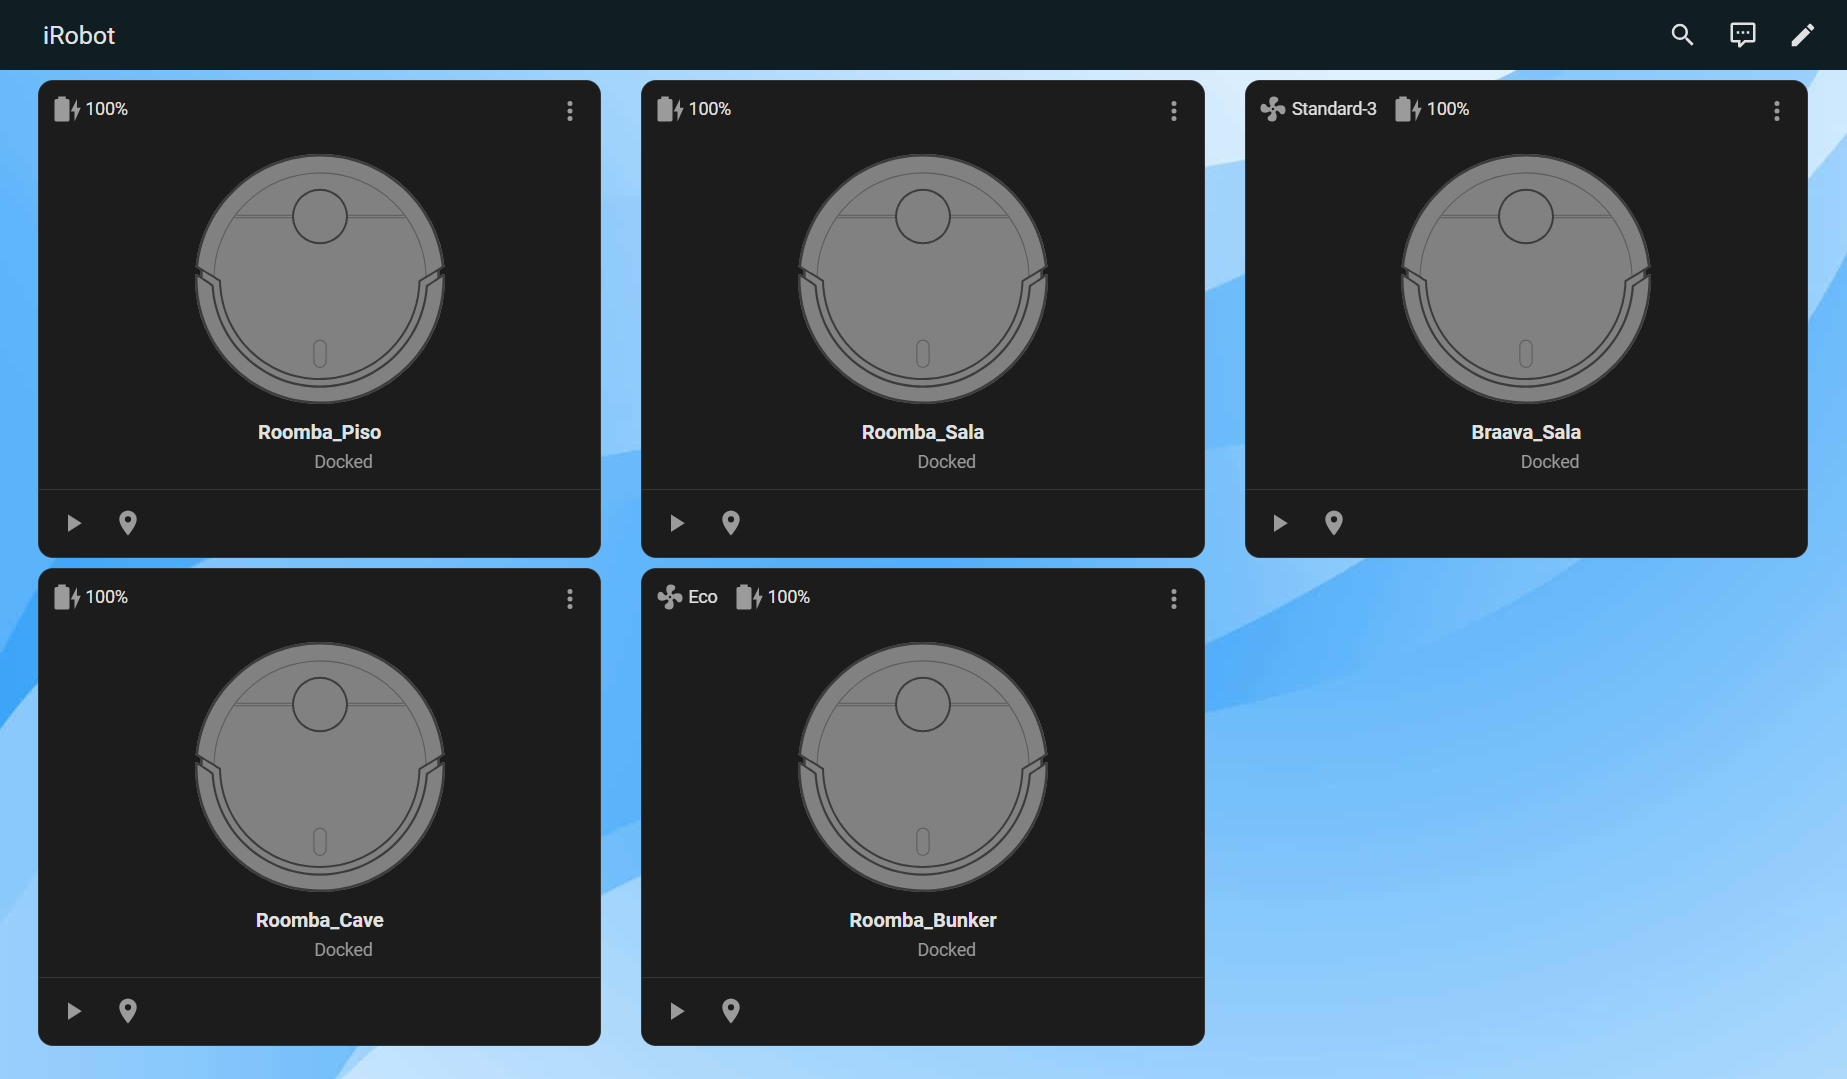
\includegraphics[width=\textwidth]{images/irobot.png}
    \caption{Dashboard Robos-Aspirador}
    \label{fig: irobot.png}
\end{figure}

A Figura~\ref{fig: irobot.png} apresenta uma dashboard do \gls{HA} dedicada à integração com dispositivos robos aspiradores. Cada cartão da dashboard representa um robô aspirador individual, com indicação clara do seu nome, estado, nível de bateria e modo de funcionamento. Os dispositivos mostrados incluem: Roomba\_Piso, Roomba\_Sala, Braava\_Sala, Roomba\_Cave e Roomba\_Bunker. Todos os aspiradores encontram-se atualmente no estado "Docked", ou seja, estacionados nas respetivas bases de carregamento, com a bateria completamente carregada (100\%). O cartão utilizado foi o "Vacuum Card", instalado a partir do \gls{HACS}.\\

\section{Integração com Alexa}

Para além das dashboards desenvolvidas, foi também implementada uma funcionalidade que permite controlar dispositivos do \gls{HA} através de comandos de voz com a assistente virtual Alexa.

A integração foi realizada de forma simples, recorrendo ao componente \textit{emulated\_hue}, que simula uma ponte \textit{Philips Hue} na rede, permitindo que a Alexa detete dispositivos expostos pelo HA. Para isso, é necessário definir o endereço IP do HA na rede local, especificar as entidades a controlar e atribuir nomes reconhecíveis por voz.

\lstset{inputencoding=ascii}
\begin{lstlisting}[language=YAML, caption={configuration.yaml}]
emulated_hue:
  type: alexa
  host_ip: ****.****.****.****  # IP da Alexa na rede local
  listen_port: 80
  expose_by_default: false
  entities:
    switch.portao_garagem:
      name: Portao
      hidden: false
\end{lstlisting}

Após inserir a configuração no ficheiro \textit{configuration.yaml} do \gls{HA}, é necessário reiniciar o sistema para aplicar as alterações. Depois do reinício, basta pedir à Alexa que procure novos dispositivos. A assistente irá detetar automaticamente o dispositivo configurado, neste caso com o nome "Portão".

Com esta configuração, ao dizer “Alexa, liga Portão” ou “Alexa, abre Portão”, a assistente interpreta o comando de voz e envia a instrução correspondente ao \gls{HA}. O ideal será utilizar o primeiro comando, uma vez que o portão da garagem está configurado como um interruptor (switch) que alterna entre os estados ligado e desligado. O \gls{HA}, ao receber o comando, ativa a entidade \textit{switch.portao\_garagem}, o que resulta na abertura do portão. Esta integração permite um controlo por voz prático, eficiente e totalmente local, sem necessidade de dependência da cloud ou de configurações adicionais externas.

Para ler estados de sensores, como por exemplo a temperatura da sala, a solução foi um pouco mais complexa. O \textit{emulated\_hue} reconhece apenas dispositivos que se comportem como interruptores, luzes, ou scripts, ou seja, não consegue ler diretamente sensores como \textit{sensor.termometro\_sala\_temperatura}.\\
Por isso, para conseguir que a Alexa "leia" a temperatura da sala, foi necessário contornar esta limitação com a seguinte abordagem:\\

Em primeiro lugar, foi criado um \textit{input\_boolean} chamado \textit{temperatura\_sala}, que simula um interruptor virtual. Este interruptor foi exposto à Alexa através do \textit{emulated\_hue}, com o nome “sala”. Assim, ao dizer “Alexa, liga sala”, ou simplesmente “Alexa, sala”,  a Alexa aciona esse interruptor, como se estivesse a ligar uma lâmpada:

\newpage

\lstset{inputencoding=ascii}
\begin{lstlisting}[language=YAML, caption={configuration.yaml}]
emulated_hue:
  type: alexa
  host_ip: ****.****.****.****  # IP da Alexa na rede local
  listen_port: 80
  expose_by_default: false
  entities:
    input_boolean.temperatura_sala:
      name: sala
      hidden: false

input_boolean:
  temperatura_sala:
    name: Perguntar temperatura
    initial: off
\end{lstlisting}

De seguida, foi criado um script no \gls{HA} que envia uma mensagem de texto-para-fala (TTS) para a Alexa com a leitura atual da temperatura. Este script utiliza a integração \textit{Alexa Media Player}, recorrendo à entidade \textit{notify.alexa\_media\_<dispositivo>} para falar diretamente através do dispositivo Alexa, utilizando a seguinte lógica:

\lstset{inputencoding=ascii}
\begin{lstlisting}[language=YAML, caption={configuration.yaml}]
sequence:
  - action: notify.alexa_media_*nome_do_dispositivo*
    data:
      message: >-
        A temperatura atual da sala e de {{
        states('sensor.netatmo_1piso_netatmo_sala_temperature') 
        }} graus.
      data:
        type: tts
alias: Alexa
description: ""
\end{lstlisting}

\vspace{-180pt}

\newpage

Por fim, foi criada uma automatização que tem como gatilho o momento em que o \textit{input\_boo-lean.temperatura\_sala} muda para o estado “on”. Quando isso acontece, a automação executa automaticamente o script anteriormente definido, fazendo com que a Alexa diga a temperatura da sala ao utilizador.

Para que o sistema funcione de forma contínua e não fique bloqueado após uma primeira utilização, a automação também inclui uma ação adicional que desliga o \textit{input\_boolean} alguns segundos depois de ser ativado. Este passo garante que a automação possa ser novamente acionada no futuro com o mesmo comando de voz.

\lstset{inputencoding=ascii}
\begin{lstlisting}[language=YAML, caption={configuration.yaml}]
alias: Alexa
description: ""
trigger:
  - platform: state
    entity_id:
      - input_boolean.temperatura_sala
    from: "off"
    to: "on"
condition: []
action:
  - service: script.alexa
    data: {}
  - service: input_boolean.turn_off
    target:
      entity_id: input_boolean.temperatura_sala
mode: single

\end{lstlisting} 

Esta abordagem permite contornar a limitação do \textit{emulated\_hue}, que não reconhece sensores, utilizando entidades compatíveis (como \textit{input\_boolean}) para simular ações compreendidas pela Alexa. Combinando um \textit{input\_boolean}, um script com TTS e uma automatização simples, é possível transformar comandos de voz em respostas inteligentes com dados em tempo real, como a leitura de temperatura, reforçando a integração entre o \gls{HA} e assistentes de voz.

\begin{table}[H]
\centering
\rowcolors{2}{gray!10}{white}
\begin{tabularx}{\textwidth}{|X|X|X|}
\hline
\textbf{Função} & \textbf{Comando} & \textbf{Entidade} \\
\hline

Abrir portão da garagem & "Alexa, liga Portão" & switch.portao\_garagem \\

Fechar portão da garagem & "Alexa, desliga Portão" & switch.portao\_garagem \\

Ler temperatura da sala & \textnormal"Alexa, sala" ou \textnormal"Alexa, liga sala" & sensor.netatmo\_1piso\_netat-mo\_sala\_temperature \\

\hline
\end{tabularx}
\caption{Funções, comandos e entidades associadas na integração da Alexa}
\end{table}
\cleardoublepage \chapter{Conclusões}\label{cap:conclusions}

O interesse por este projeto surgiu da vontade de explorar o potencial da domótica aliada à integração de sistemas inteligentes, com enfoque numa plataforma \gls{OS} como o \gls{HA}. Desde o início, o desafio foi compreender e controlar as diferentes valências de uma casa inteligente, desde a gestão energética à climatização, videovigilância, automação de estores e integração de sensores ambientais.

Ao longo do desenvolvimento, foi necessário realizar uma pesquisa aprofundada sobre os dispositivos utilizados, aprender as boas práticas da configuração com \gls{YAML} e enfrentar desafios técnicos, como a integração de equipamentos distintos e a personalização de dashboards funcionais e intuitivos. A introdução do \gls{HACS} e de integrações como a \textit{Huawei Solar}, \textit{Reolink}, \textit{Daikin}, \textit{Shelly}, \textit{Netatmo} e \textit{iRobot} permitiu criar um sistema robusto e flexível, adaptado às necessidades reais de uma habitação moderna.

Apesar das dificuldades encontradas, o projeto revelou-se uma experiência enriquecedora. Não só permitiu aplicar conhecimentos técnicos adquiridos ao longo da licenciatura, como também impulsionou novas aprendizagens em áreas como automação residencial, monitorização energética e interfaces homem-máquina. O resultado é uma solução funcional, prática e escalável, capaz de evoluir com as necessidades do utilizador.

Em suma, este trabalho demonstrou a viabilidade de construir um sistema de casa inteligente totalmente integrado, centralizado, personalizável e de baixo custo, utilizando apenas ferramentas de código aberto e conectividade Wi-Fi. O projeto reforça ainda a importância da interoperabilidade entre dispositivos e da usabilidade no contexto da domótica, abrindo caminho a futuros desenvolvimentos e integrações ainda mais avançadas.


\newpage
Adicionalmente, importa referir uma questão de segurança.


É de elevada importância, considerando as boas práticas de segurança, utilizar protocolos \textit{TLS/SSL} integrando add-ons como o \textit{Duck DNS} que inclui configurações automáticas \textit{HTTPS} com certificados \textit{Let's Encrypt}, garantindo a encriptação das comunicações e proteção acrescida contra exposição de dados e possíveis ataques, ex. \textit{man-in-the-middle (MITM)}.


Da mesma forma, a implementação de uma rede WiFi dedicada permite isolar os dispositivos \gls{IoT} na sua própria rede, reduzindo o risco de estes serem comprometidos e, potencialmente, darem acesso à rede principal e a outros hosts o que representaria uma falha grave de segurança. Esta solução, ao endereçar o tráfego \gls{IoT} para uma rede separada, liberta a rede principal que terá um desempenho melhorado especialmente se tivermos um número elevado de dispositivos ligados. A gestão e a resolução de problemas relacionados com os dispositivos \gls{IoT} acaba por ser facilitada uma vez que podem ser aplicadas e/ou testadas políticas específicas sem afetar a rede principal.

Durante o desenvolvimento deste projeto, foi também elaborado um artigo científico detalhado sobre a plataforma \gls{HA}, com especial foco na estrutura do sistema e nas dashboards criadas. Este artigo descreve a organização do sistema de casa inteligente, as funcionalidades implementadas e a integração entre os vários componentes. O trabalho foi submetido à 13th edition of the Technological Ecosystems for Enhancing Multiculturality (TEEM) e à 12th International Electronic Conference on Sensors and Applications, com o objetivo de partilhar os resultados alcançados e contribuir para a comunidade científica na área da automação residencial e IoT.


\cleardoublepage \input{chapters/cap06}

% Bibliografia
\printbibliography

% Apêndices
\appendix

% Numeração especial para apêndices
\pretocmd{\chapter}{%
  \clearpage
  \pagenumbering{arabic}%
  \renewcommand*{\thepage}{\thechapter\arabic{page}}%
}{}{}

% Inclusão dos apêndices
% No corpo do documento, onde for inserir o apêndice
\chapter{Proposta Original do Projeto}
\label{apendice1}

A proposta original do projeto encontra-se nas páginas seguintes.

\clearpage
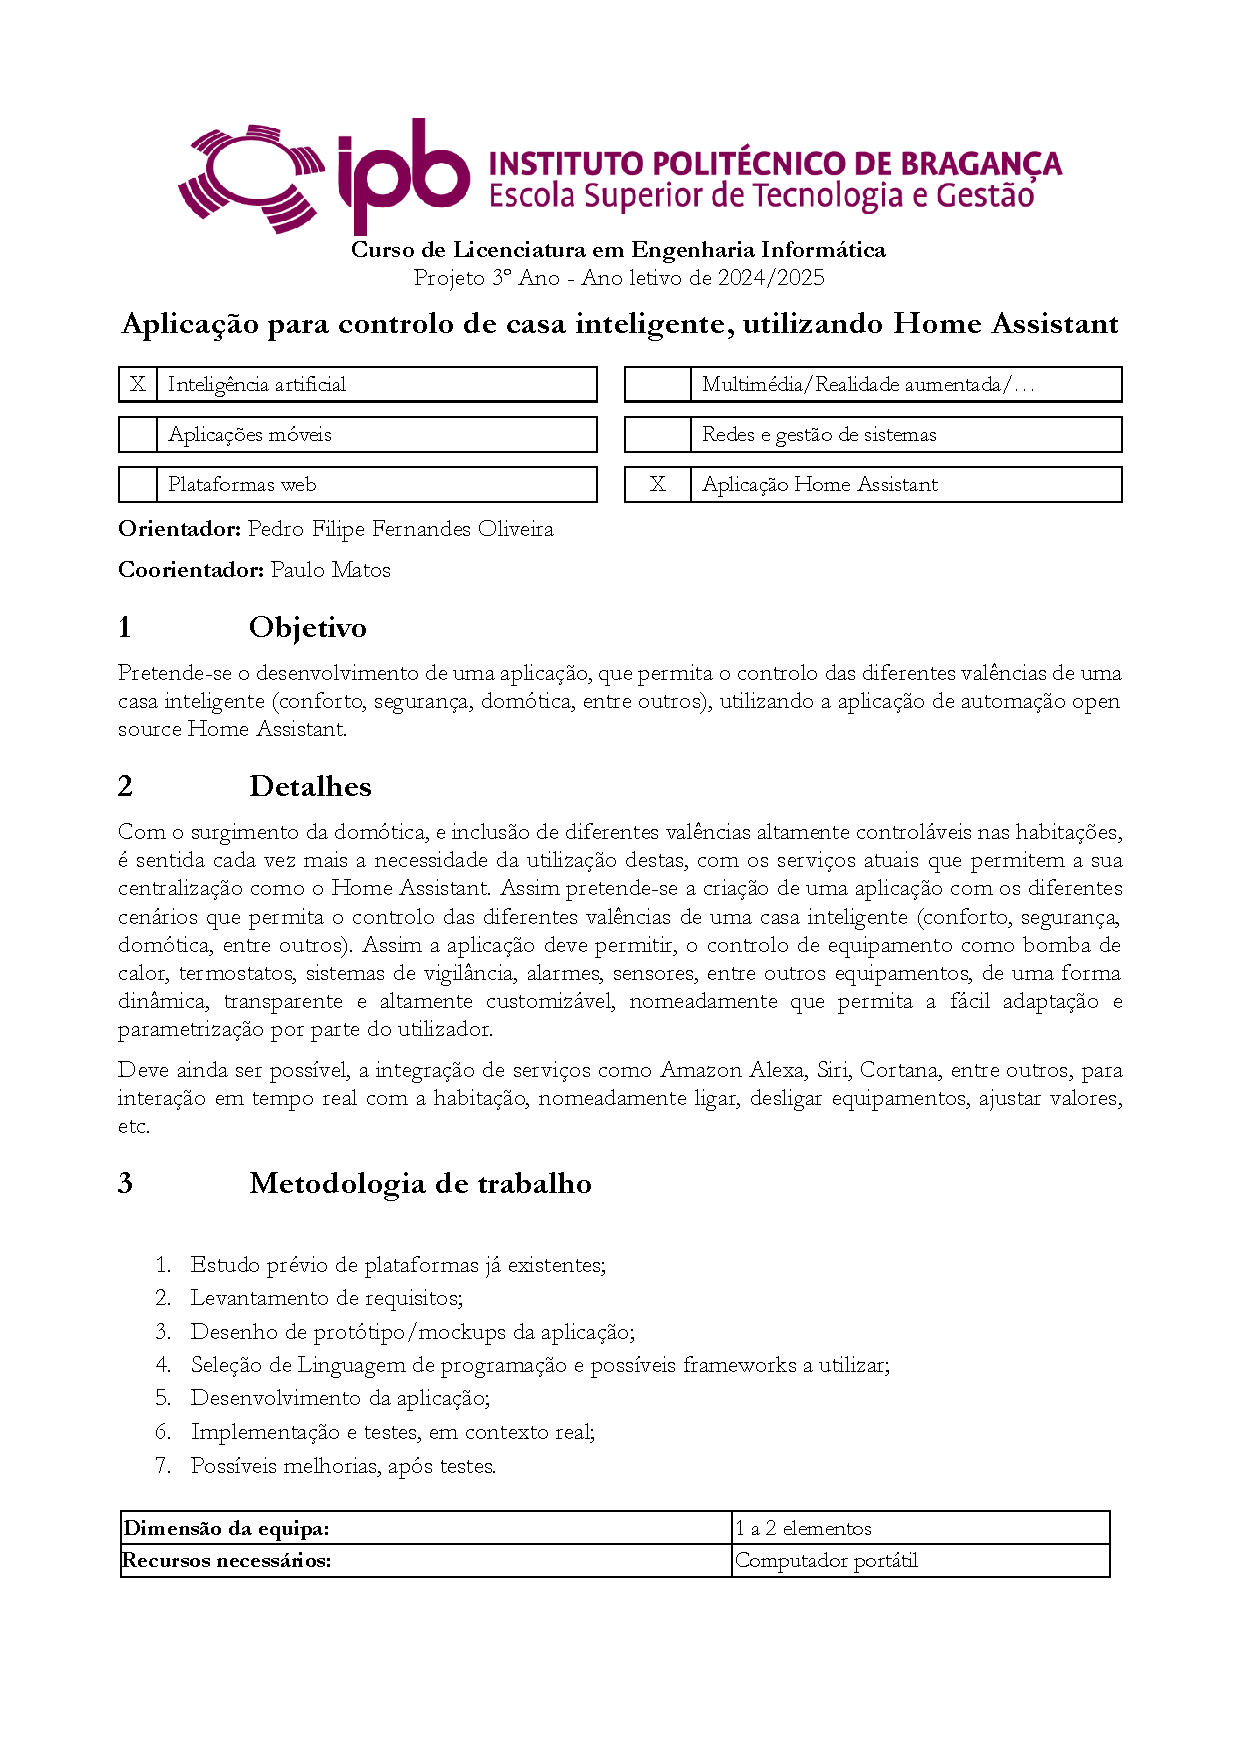
\includepdf[pages=-,pagecommand={}]{etc/PropostaProjeto.pdf}
\chapter{Apêndice B – Listagens de Código e
Detalhes Técnicos
}
\label{apendice2}

Os códigos desenvolvidos e os detalhes técnicos do projeto podem ser encontrados no repositório disponível em: \url{https://gitlab.estig.ipb.pt/projetos_ei/2025_p18_homeassistant}.

\section{Código das bombas}

\lstset{inputencoding=ascii}
\begin{lstlisting}[language=YAML, caption={pumps.yaml}]
# Pumps mostram 0W em standby
- sensor:
    - name: "Bomba AQS Filtered Power"
      unit_of_measurement: "W"
      device_class: power
      state_class: measurement
      state: >
        
          0
        
          {{ states('sensor.bomba_aqs_power') }}
        

    - name: "Bomba Calor Filtered Power"
      unit_of_measurement: "W"
      device_class: power
      state_class: measurement
      state: >
        
          0
        
          {{ states('sensor.bomba_calor_power') }}
        

    - name: "Heat Pump Daily Consumption"
      unit_of_measurement: "kWh"
      device_class: energy
      state_class: total_increasing
      state: >
        {{ (
          states('sensor.altherma_climatecontrol_cooling_daily_electrical_consumption') | float(0) +
          states('sensor.altherma_climatecontrol_heating_daily_electrical_consumption') | float(0)
        ) | round(2) }}

\end{lstlisting}


\section{Código dos carregadores}

\lstset{inputencoding=ascii}
\begin{lstlisting}[language=YAML, caption={ev.yaml}]
# EV mostra 0W em standby
- sensor:
    - name: "EV_16 Filtered Power"
      unit_of_measurement: "W"
      device_class: power
      state_class: measurement
      state: >
        
          0
        
          {{ states('sensor.ev_16a_power') }}
        

    - name: "EV_32 Filtered Power"
      unit_of_measurement: "W"
      device_class: power
      state_class: measurement
      state: >
        
          0
        
          {{ states('sensor.ev_32a_power') }}
        

\end{lstlisting}

\section{Código das notificações}

\lstset{inputencoding=ascii}
\begin{lstlisting}[language=YAML, caption={notifications.yaml}]
# Sensor de Alerta
- sensor:
    - name: "Estado de Alerta"
      unique_id: estado_alerta
      state: >
        
          Open gate
        
          Rain
        
          High CO2
        
          High Noise
        
          Robot cleaning
        
          Heat pump connected
        
          DHW pump connected
        
          Strong wind
        
          Negative temperature
        
          High humidity
        
          Low humidity
        
          All clean
        


\end{lstlisting}


\section{Código do consumo da casa}

\lstset{inputencoding=ascii}
\begin{lstlisting}[language=YAML, caption={house\_consumption.yaml}]
#Necessario para o card energy
- sensor:
    - name: "Consumo da Casa novo"
      unit_of_measurement: "W"
      device_class: power
      state_class: measurement
      state: >
        
        
        

        
          unavailable
        
          
          

          
          
          
          

          
          {{ consumo | round(2) }}
        


\end{lstlisting}

\section{Código do estado exportação da rede}

\lstset{inputencoding=ascii}
\begin{lstlisting}[language=YAML, caption={grid.yaml}]
# Botao de exportacao
- sensor:
    - name: "Exportacao_Status"
      unique_id: exportacao_status
      state: >
        

        
          ultra
        
          high
        
          medium
        
          low
        



\end{lstlisting}



\section{Código do conversão do gráfico para 15min}

\lstset{inputencoding=ascii}
\begin{lstlisting}[language=YAML, caption={conversion\_grafic\_15min.yaml}]
#Conversao para graficos e atualizacoes em 15 min
- trigger:
    - platform: time_pattern
      minutes: "/15"
  sensor:
    - name: "Consumo da Casa em kW (15min)"
      unit_of_measurement: "kW"
      device_class: power
      state_class: measurement
      state: >
        {{ (states('sensor.consumo_da_casa_novo') | float(0) / 1000) | round(2) }}

    - name: "Produção Solar em kW (15min)"
      unit_of_measurement: "kW"
      device_class: power
      state_class: measurement
      state: >
        {{ (states('sensor.solar_total') | float(0) / 1000) | round(2) }}

    - name: "EV16 Power em kW (15min)"
      unit_of_measurement: "kW"
      device_class: power
      state_class: measurement
      state: >
        {{ (states('sensor.ev_16a_power') | float(0) / 1000) | round(2) }}

    - name: "EV32 Power em kW (15min)"
      unit_of_measurement: "kW"
      device_class: power
      state_class: measurement
      state: >
        {{ (states('sensor.ev_32a_power') | float(0) / 1000) | round(2) }}


\end{lstlisting}

\section{Código das conversões}

\lstset{inputencoding=ascii}
\begin{lstlisting}[language=YAML, caption={conversions.yaml}]
 # CONVERSOES PARA OS GRAFICOS
- sensor:
    - name: "Consumo da Casa em kW"
      unit_of_measurement: "kW"
      device_class: power
      state_class: measurement
      state: >
        {{ (states('sensor.consumo_da_casa_novo') | float(0) / 1000) | round(2) }}

    - name: "Produção Solar em kW"
      unit_of_measurement: "kW"
      device_class: power
      state_class: measurement
      state: >
        {{ (states('sensor.solar_total') | float(0) / 1000) | round(2) }}

    - name: "EV16 Power em kW"
      unit_of_measurement: "kW"
      device_class: power
      state_class: measurement
      state: >
        {{ (states('sensor.ev_16a_power') | float(0) / 1000) | round(2) }}

    - name: "EV32 Power em kW"
      unit_of_measurement: "kW"
      device_class: power
      state_class: measurement
      state: >
        {{ (states('sensor.ev_32a_power') | float(0) / 1000) | round(2) }}


\end{lstlisting}

\section{Código do solar}

\lstset{inputencoding=ascii}
\begin{lstlisting}[language=YAML, caption={conversions.yaml}]
# Saida de casa Solar
- sensor:
    - name: "PV1 Master Power"
      unit_of_measurement: "W"
      device_class: power
      state_class: measurement
      state: >
        {{ (states('sensor.inverter_pv_1_current') | float(0) * states('sensor.inverter_pv_1_voltage') | float(0)) | round(2) }}

    - name: "PV2 Master Power"
      unit_of_measurement: "W"
      device_class: power
      state_class: measurement
      state: >
        {{ (states('sensor.inverter_pv_2_current') | float(0) * states('sensor.inverter_pv_2_voltage') | float(0)) | round(2) }}

    - name: "PV1 Slave Power"
      unit_of_measurement: "W"
      device_class: power
      state_class: measurement
      state: >
        {{ (states('sensor.inverter_pv_1_voltage_2') | float(0) * states('sensor.inverter_pv_1_current_2') | float(0)) | round(2) }}

# Soma dos 2 inversores
    - name: "Solar Total"
      unit_of_measurement: "W"
      device_class: power
      state_class: measurement
      state: >
        
        
        {{ a + b }}
        
    - name: "Soma dos 3 Solares"
      unit_of_measurement: "W"
      state: >
          
          
          
          {{ (s1 + s2 + s3) | round(2) }}

\end{lstlisting}
\chapter{Apêndice C – Diagramas desenvolvidos
}


\section{Diagrama do cenário de aplicação}




\begin{figure}[H]
    \centering
    \includegraphics[width=0.7\textwidth]{Diagram_HA.png}
    \caption{Diagrama do cenário de aplicação}
    \label{fig:Diagram_HA.png}
\end{figure}

\newpage

\section{Diagrama do consumo}



\begin{figure}[H]
    \centering
    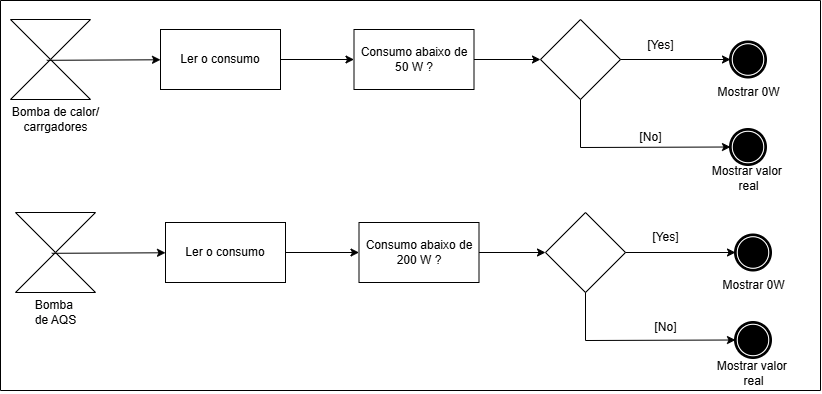
\includegraphics[width=\textwidth]{consumo.png}
    \caption{Diagrama do consumo}
    \label{fig:consumo.png}
\end{figure}


\newpage

\section{Diagrama da exportação da rede}


\begin{figure}[H]
    \centering
    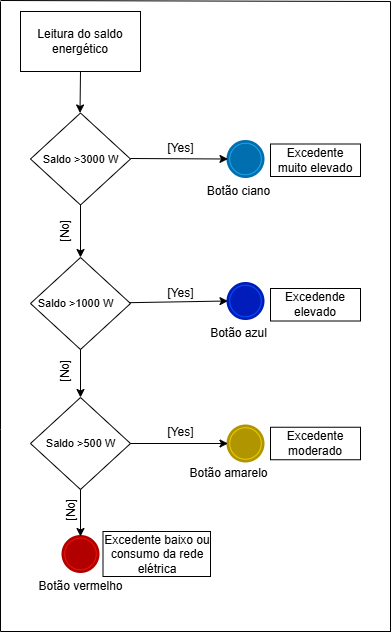
\includegraphics[width=0.5\textwidth]{images/Saldo_Botao_Energetico_diagrama.drawio.png}
    \caption{Diagrama da exportação da rede}
    \label{fig:Saldo_Botao_Energetico_diagrama.drawio.png}
\end{figure}

\chapter{Apêndice D – Artigo submetido nas conferências}

O artigo científico submetido às conferências **13th TEEM** e **12th International Electronic Conference on Sensors and Applications** encontra-se nas páginas seguintes.

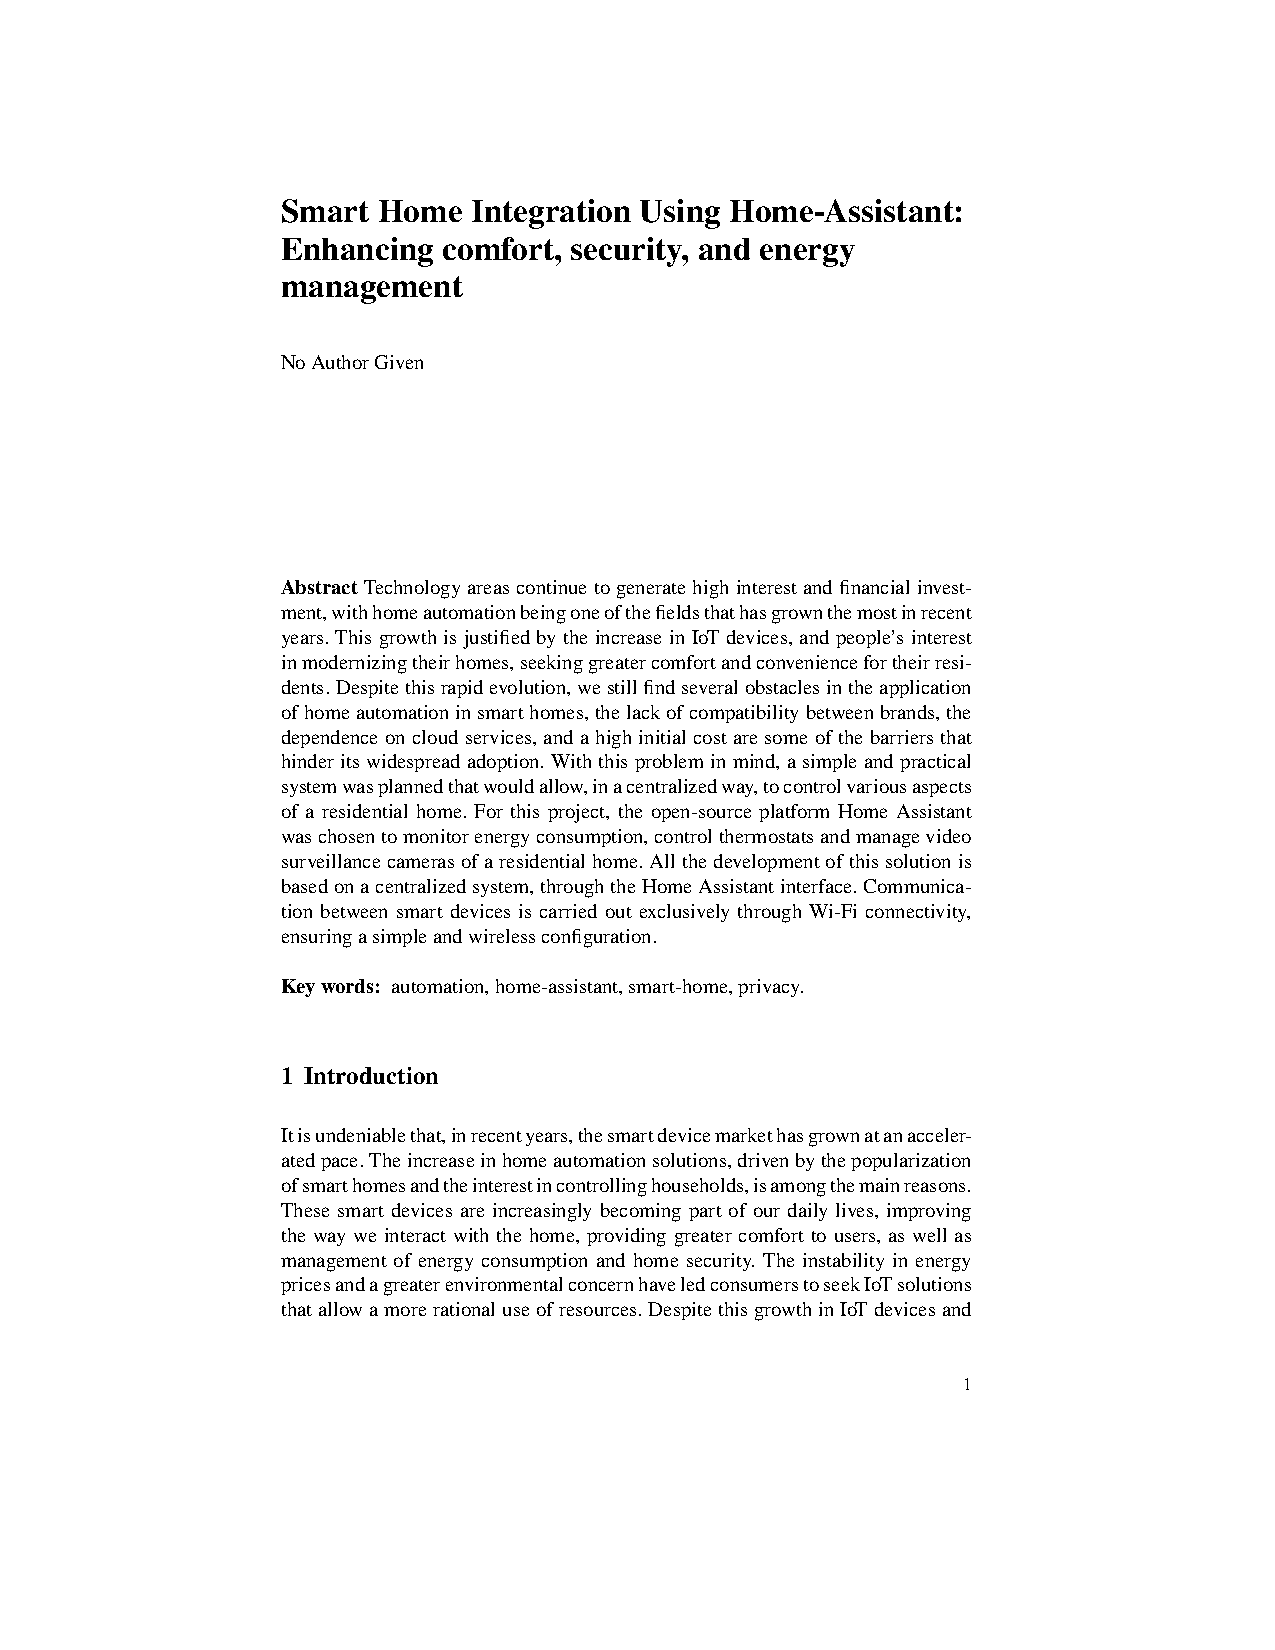
\includepdf[pages=-,pagecommand={}]{etc/Paper_TEEM_2025_HomeAssistant.pdf}


\end{document}
